% This file is intended to be included from your main LaTeX document, e.g. via % This file is intended to be included from your main LaTeX document, e.g. via % This file is intended to be included from your main LaTeX document, e.g. via % This file is intended to be included from your main LaTeX document, e.g. via \input{assets/methodology_three_stage_workflow.tex}
% Figure paths assume the main document's working directory contains assets/ as a sibling (adjust if needed).

\section{4. Methodology: The Three-Stage Workflow}
To investigate the connection between registration error and uncertainty, we built a modular pipeline designed to bypass the Correspondence Paradox. Instead of attempting to infer uncertainty directly from unknown correspondences, we generate synthetic deformations with known ground truth and then train a supervised regression model to predict the resulting registration error map.

Our pipeline has three distinct phases: (I) Ground Truth Data Generation, (II) Registration Error Map Generation, and (III) Supervised Error Map Training.

\subsection{Phase 1: Ground Truth Generation}
In Phase~1 we generate synthetic 2D registration triplets $(I_{\text{fixed}}, I_{\text{warped}}, \phi_{\text{true}})$ from raw IXI slices. Each synthetic sample is produced by applying a random affine deformation followed by a random elastic deformation to the slice geometry. The ground-truth displacement field is computed explicitly from the transformed sampling grid, enabling pixelwise supervision in later stages.

\paragraph{Random deformation and deformation field.}
Let $g_{\text{identity}}(u)$ denote the identity sampling grid at pixel location $u$, and let $g_{\text{transformed}}(u)$ be the sampling grid after applying the composed transforms. The synthetic displacement field is defined as
\[
  \phi_{\text{true}}(u) = g_{\text{transformed}}(u) - g_{\text{identity}}(u),
]
and the corresponding warped image $I_{\text{warped}}$ is obtained by the same transform used to compute $\phi_{\text{true}}$. The pipeline also defines an interior supervision region by excluding a boundary margin of $10$ pixels, producing a binary $\mathrm{valid\_mask}$ used to focus training on reliable pixels.

\paragraph{Quality control (QC) and dataset stability.}
To avoid degenerate deformations, each candidate sample undergoes QC acceptance checks on deformation magnitude and on warped intensity statistics. Candidate samples are attempted up to a fixed number of times; if QC still fails, the sample can be saved with $\mathrm{qc\_passed}=false$ (useful for optional regeneration/cleanup).

Key acceptance constraints include:
\begin{itemize}
  \item Affine parameters are constrained by pre-defined ranges for scale, rotation, and translation in pixels.
  \item Elastic deformation is constrained via the number of control points, maximum displacement magnitude, and application probability.
  \item Rejection if $|\phi|$ exceeds configured thresholds either on the interior band or globally.
  \item Rejection if the warped image is overly dark (a minimum ratio constraint on mean intensity).
\end{itemize}

\paragraph{Ground truth triplets (visual inspection).}
Figure~\ref{fig:triplet_examples} shows representative synthetic triplets for the Train split: fixed image, warped image, and the deformation magnitude $\|\phi\|$ in pixels.

\begin{figure}[t]
  \centering
  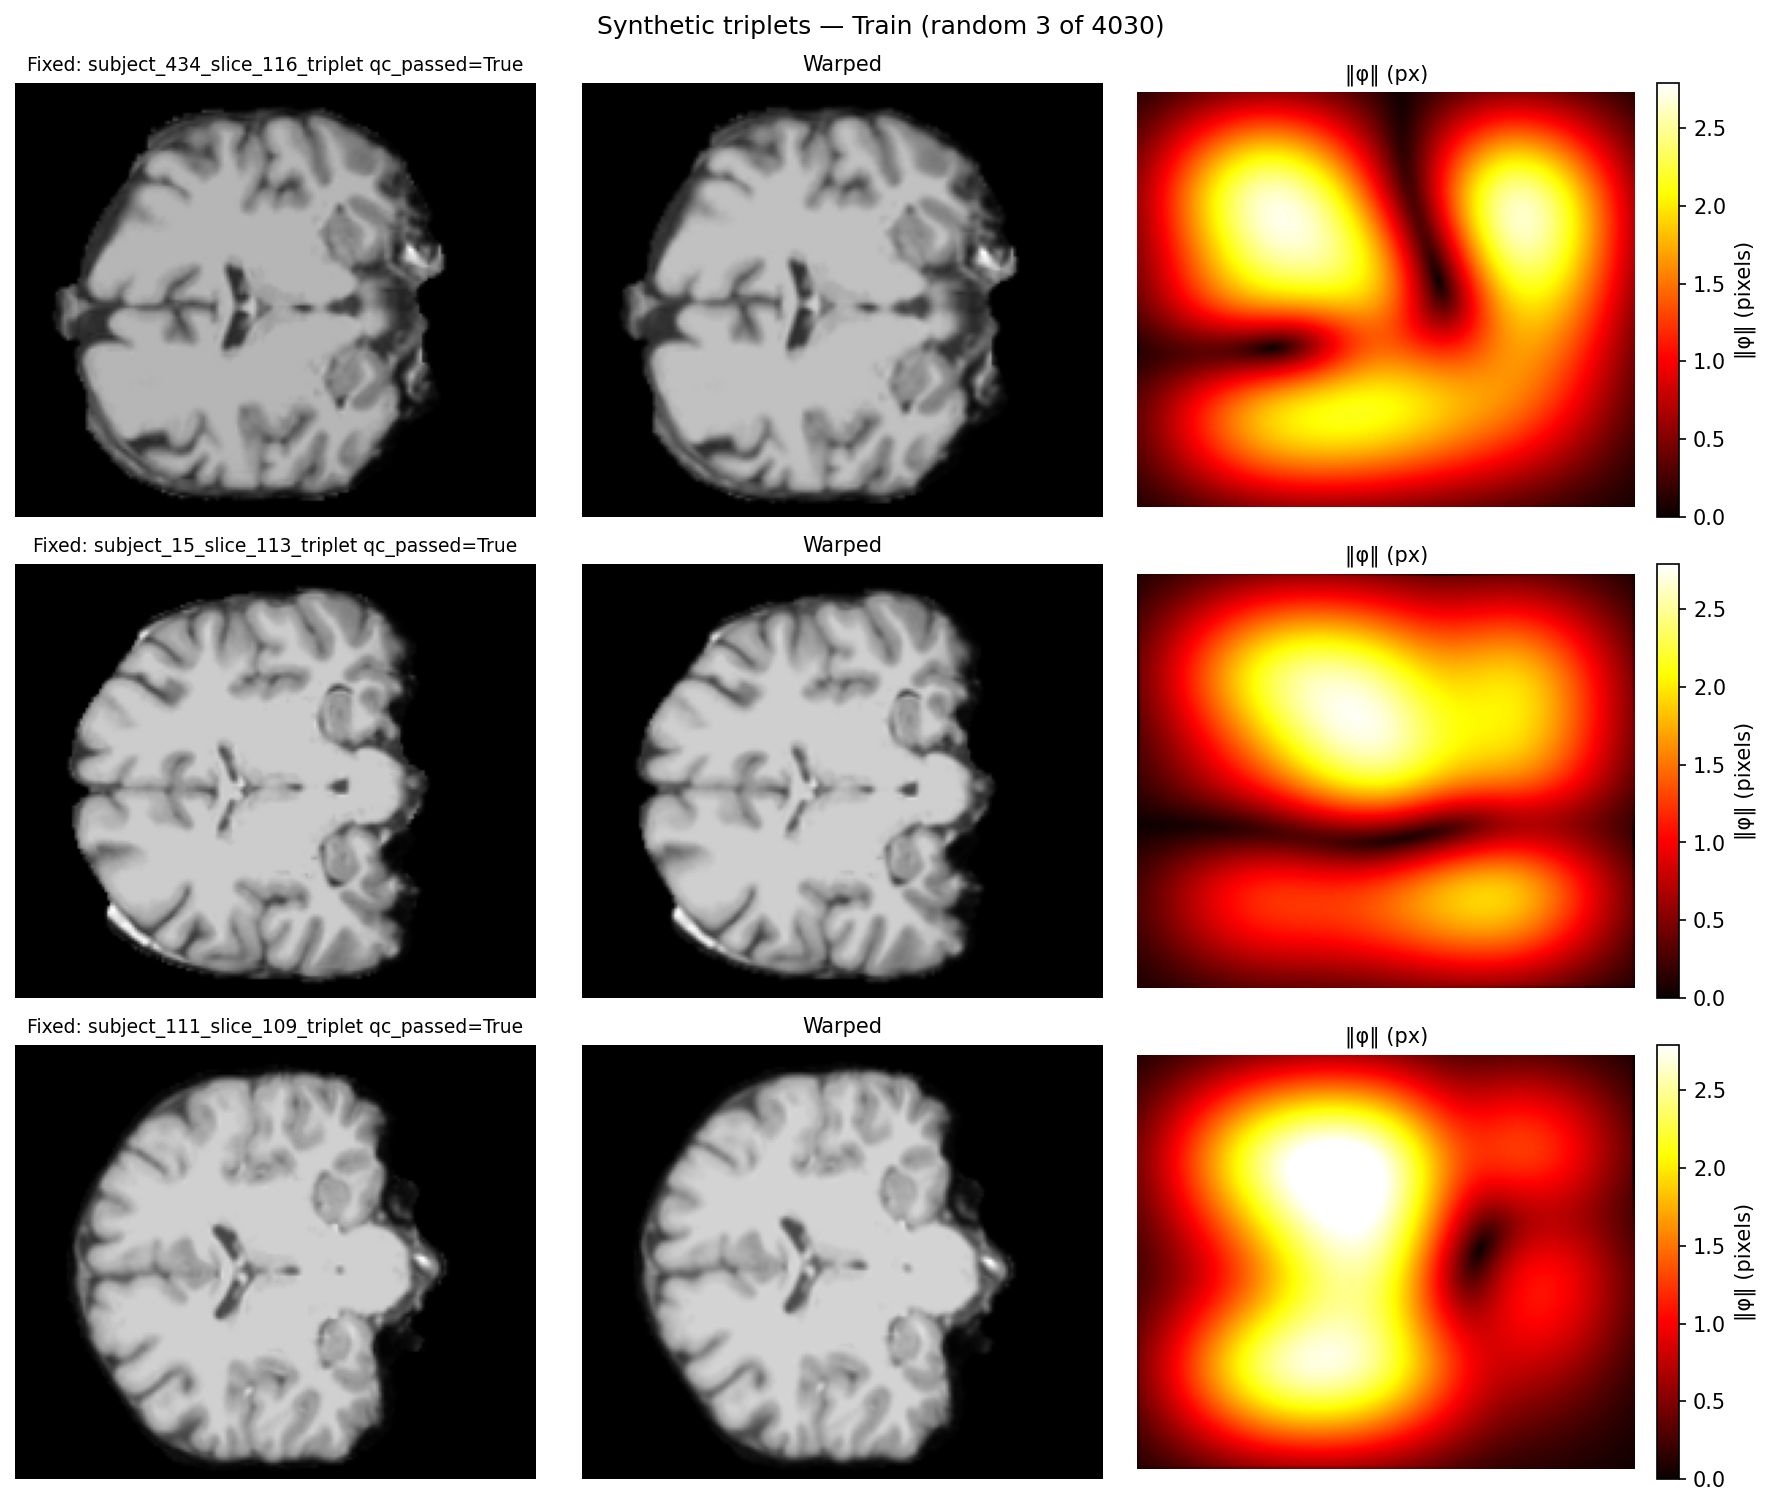
\includegraphics[width=0.95\linewidth]{assets/images/synthetic/ixi_synth_mtrain.png}
  \caption{Synthetic registration triplets generated in Phase~1 (fixed image, warped image, and deformation magnitude $\|\phi\|$).}
  \label{fig:triplet_examples}
\end{figure}

To support qualitative analysis across ``easy'' and ``hard'' deformation regimes, we additionally select min/median/max examples by a scalar $\phi$ statistic (default: mean deformation magnitude over the slice). Figure~\ref{fig:triplet_minmedmax} illustrates these representative extremes.

\begin{figure}[t]
  \centering
  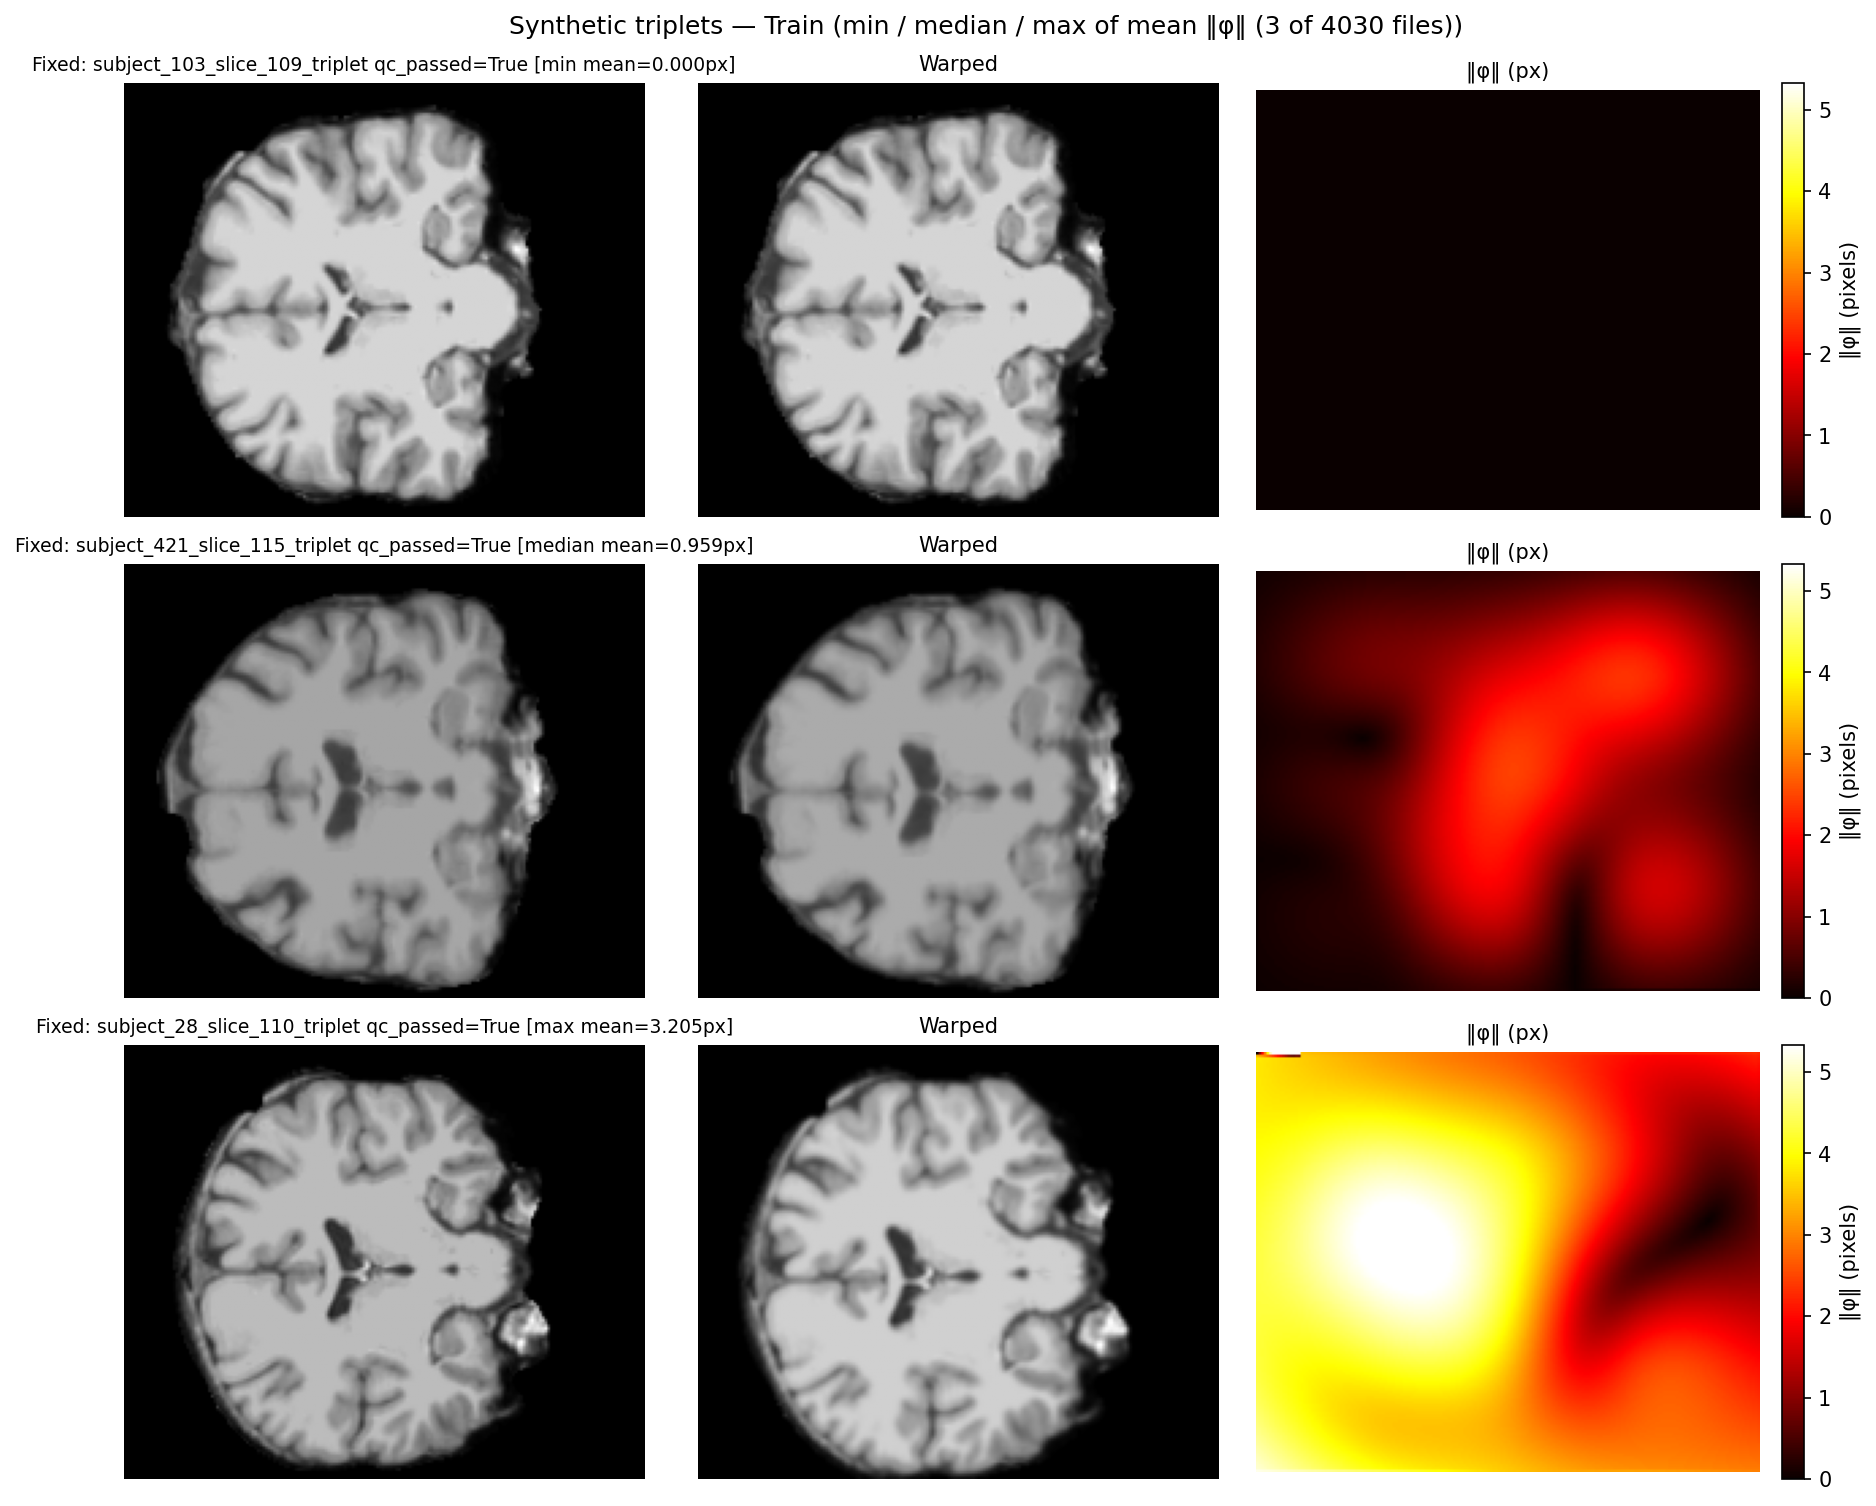
\includegraphics[width=0.95\linewidth]{assets/images/synthetic/ixi_synth_mtrain_minmedmax.png}
  \caption{Min/median/max synthetic triplets by deformation magnitude $\|\phi\|$ for the Train split.}
  \label{fig:triplet_minmedmax}
\end{figure}

\subsection{Phase 2: Registration Error Map Generation}
Phase~2 converts synthetic triplets into supervised scalar error maps by running UniGradICON to predict a deformation field and comparing it with the known synthetic ground truth.

\paragraph{UniGradICON fiver generation.}
For each triplet in each split (Train/Val/Test/Atlas), we:
\begin{itemize}
  \item Run UniGradICON to infer the deformation in the ICON coordinate system.
  \item Convert the predicted deformation back to the original 2D pixel grid to obtain $\phi_{\text{pred}}$ in pixel units.
  \item Compute the residual displacement $\phi_{\text{diff}}=\phi_{\text{true}}-\phi_{\text{pred}}$.
  \item Produce a scalar error map
  \[
    e(u) = \|\phi_{\text{true}}(u) - \phi_{\text{pred}}(u)\|_2
         = \sqrt{\Delta\phi_x(u)^2 + \Delta\phi_y(u)^2}.
  \]
\end{itemize}

The output fiver files ($\ast$$_\mathrm{fiver}$.npz) store, for each pixel, the fixed/warped images, $\phi_{\text{true}}$, $\phi_{\text{pred}}$, $\phi_{\text{diff}}$, and the scalar error map $e(u)$. Importantly, they also store $\mathrm{valid\_mask}$ and the QC flag propagated from Phase~1, enabling masked training later.

\paragraph{Phase~2 visualization.}
Figures~\ref{fig:unigrad_train} and \ref{fig:unigrad_train_minmedmax} show the UniGradICON-derived quantities for representative Train samples, including $\|\phi_{\text{true}}\|$, $\|\phi_{\text{pred}}\|$, and the scalar error map $\|\phi_{\text{true}}-\phi_{\text{pred}}\|$.

\begin{figure}[t]
  \centering
  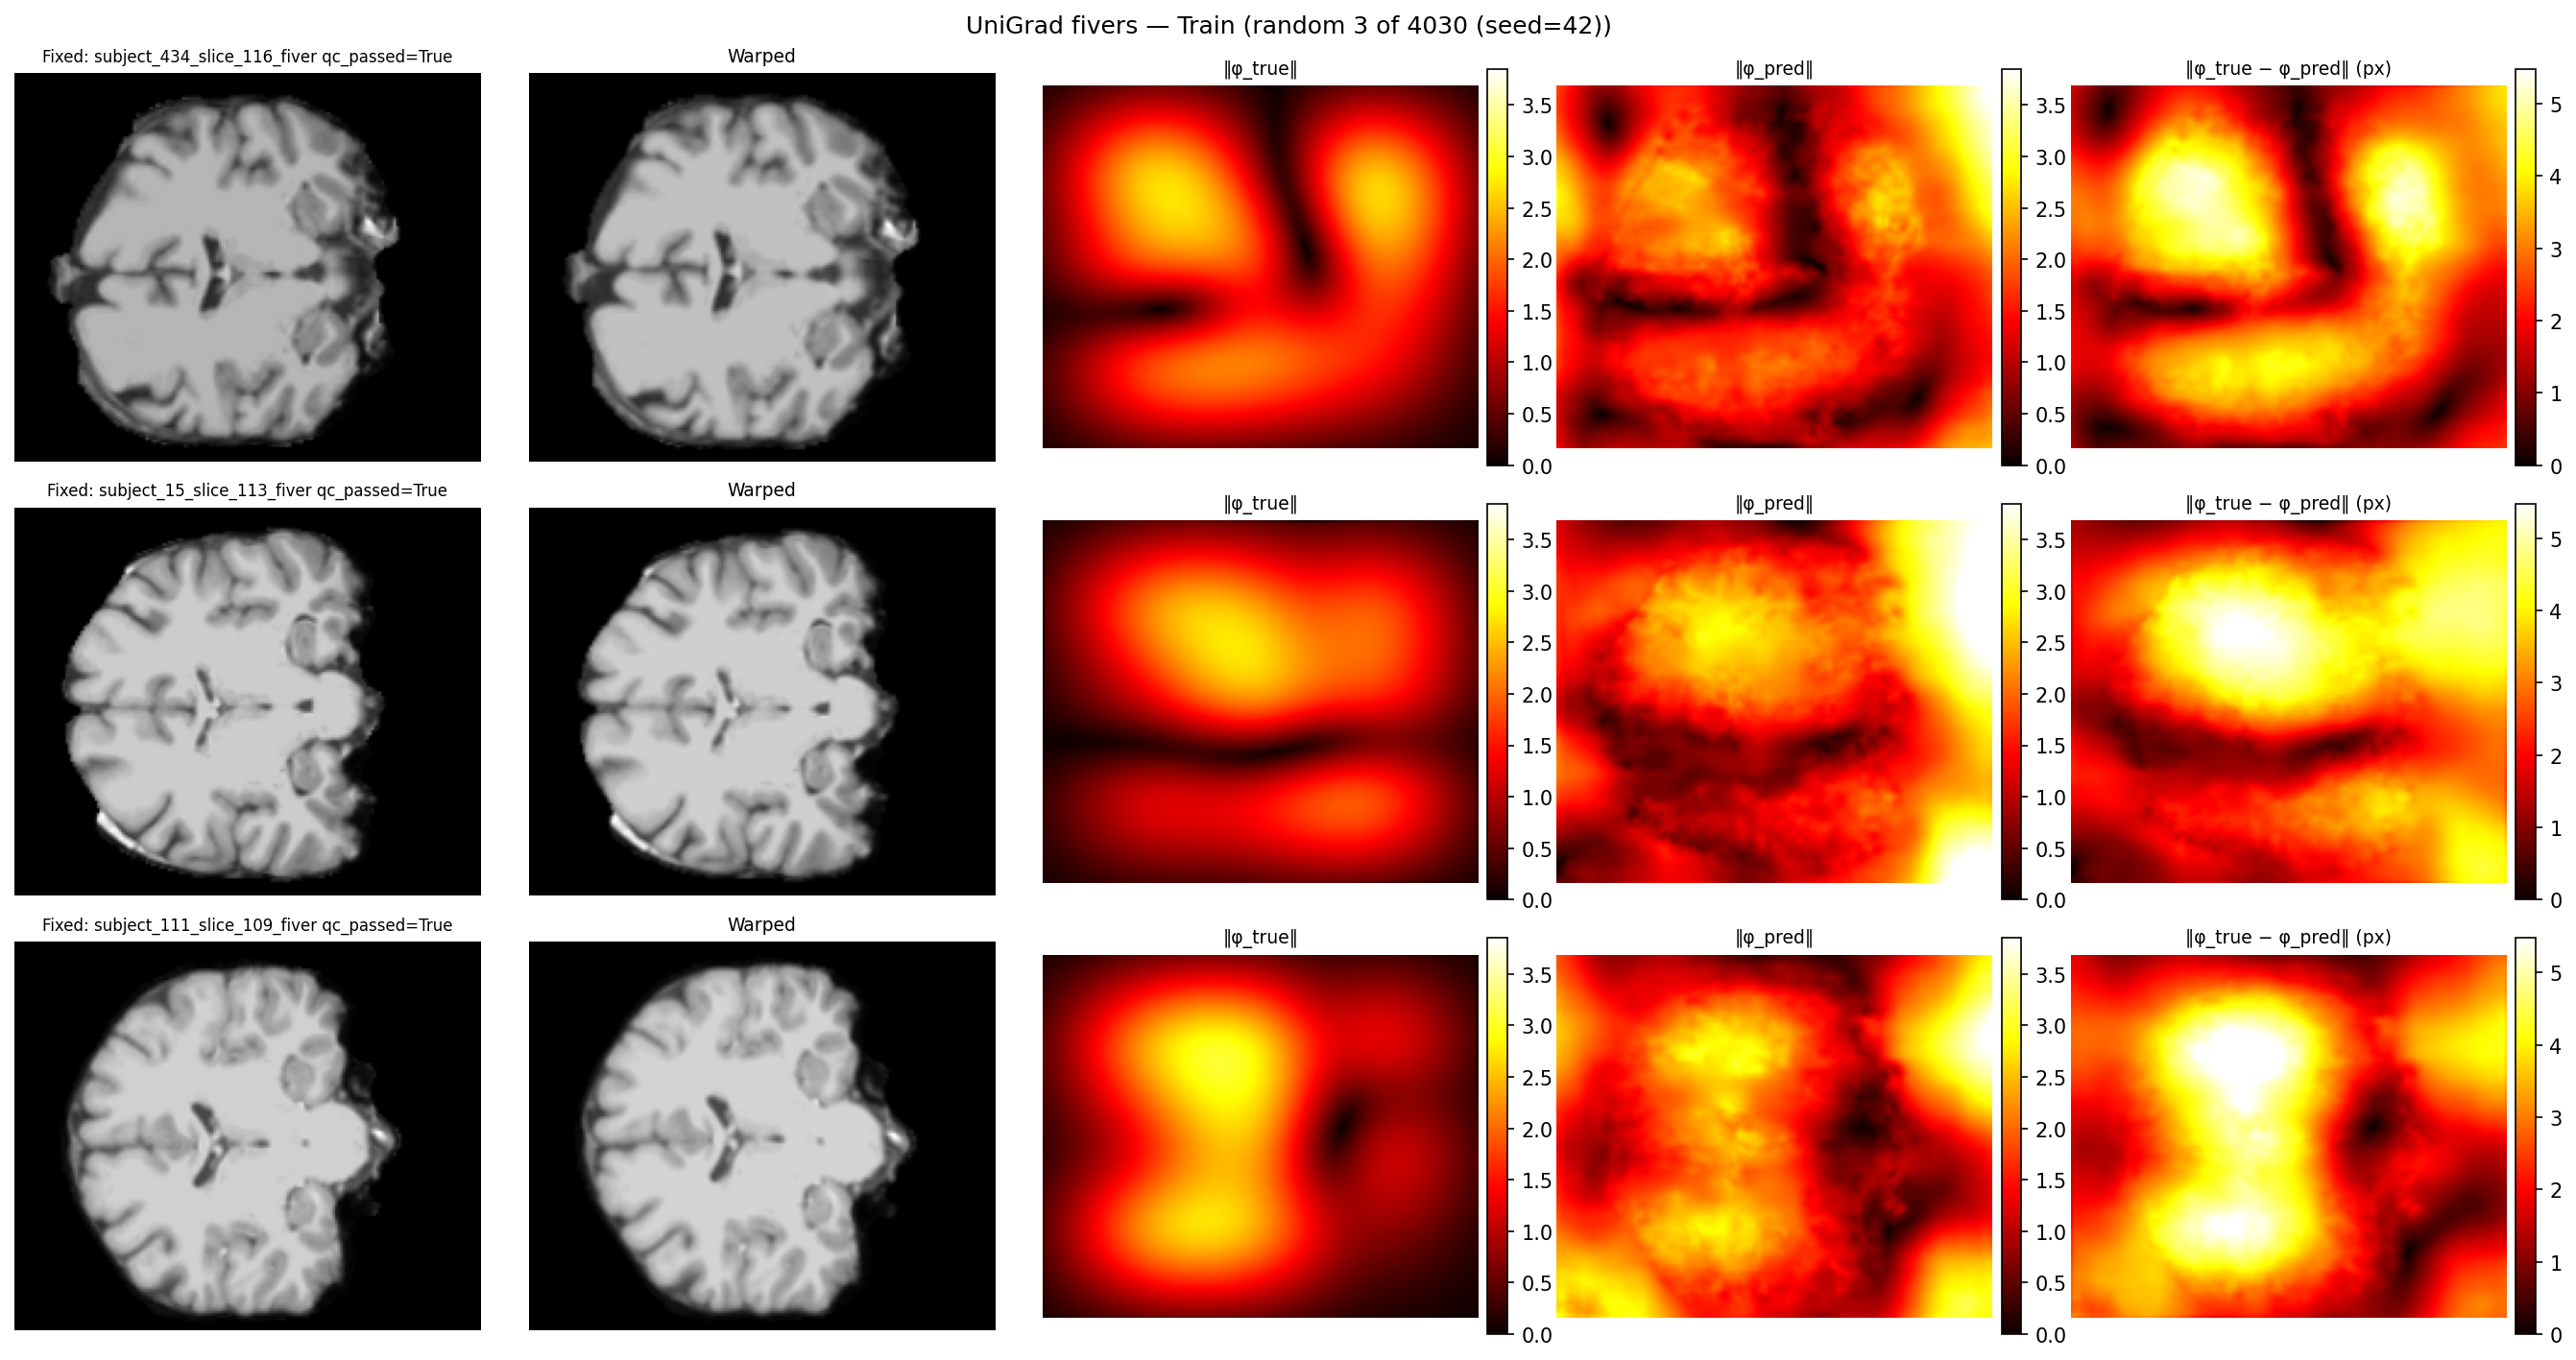
\includegraphics[width=0.95\linewidth]{assets/images/unigrad/ixi_unigrad_train.png}
  \caption{UniGradICON fiver visualization in Phase~2 for the Train split (including $\|\phi_{\text{true}}\|$, $\|\phi_{\text{pred}}\|$, and the scalar error map).}
  \label{fig:unigrad_train}
\end{figure}

\begin{figure}[t]
  \centering
  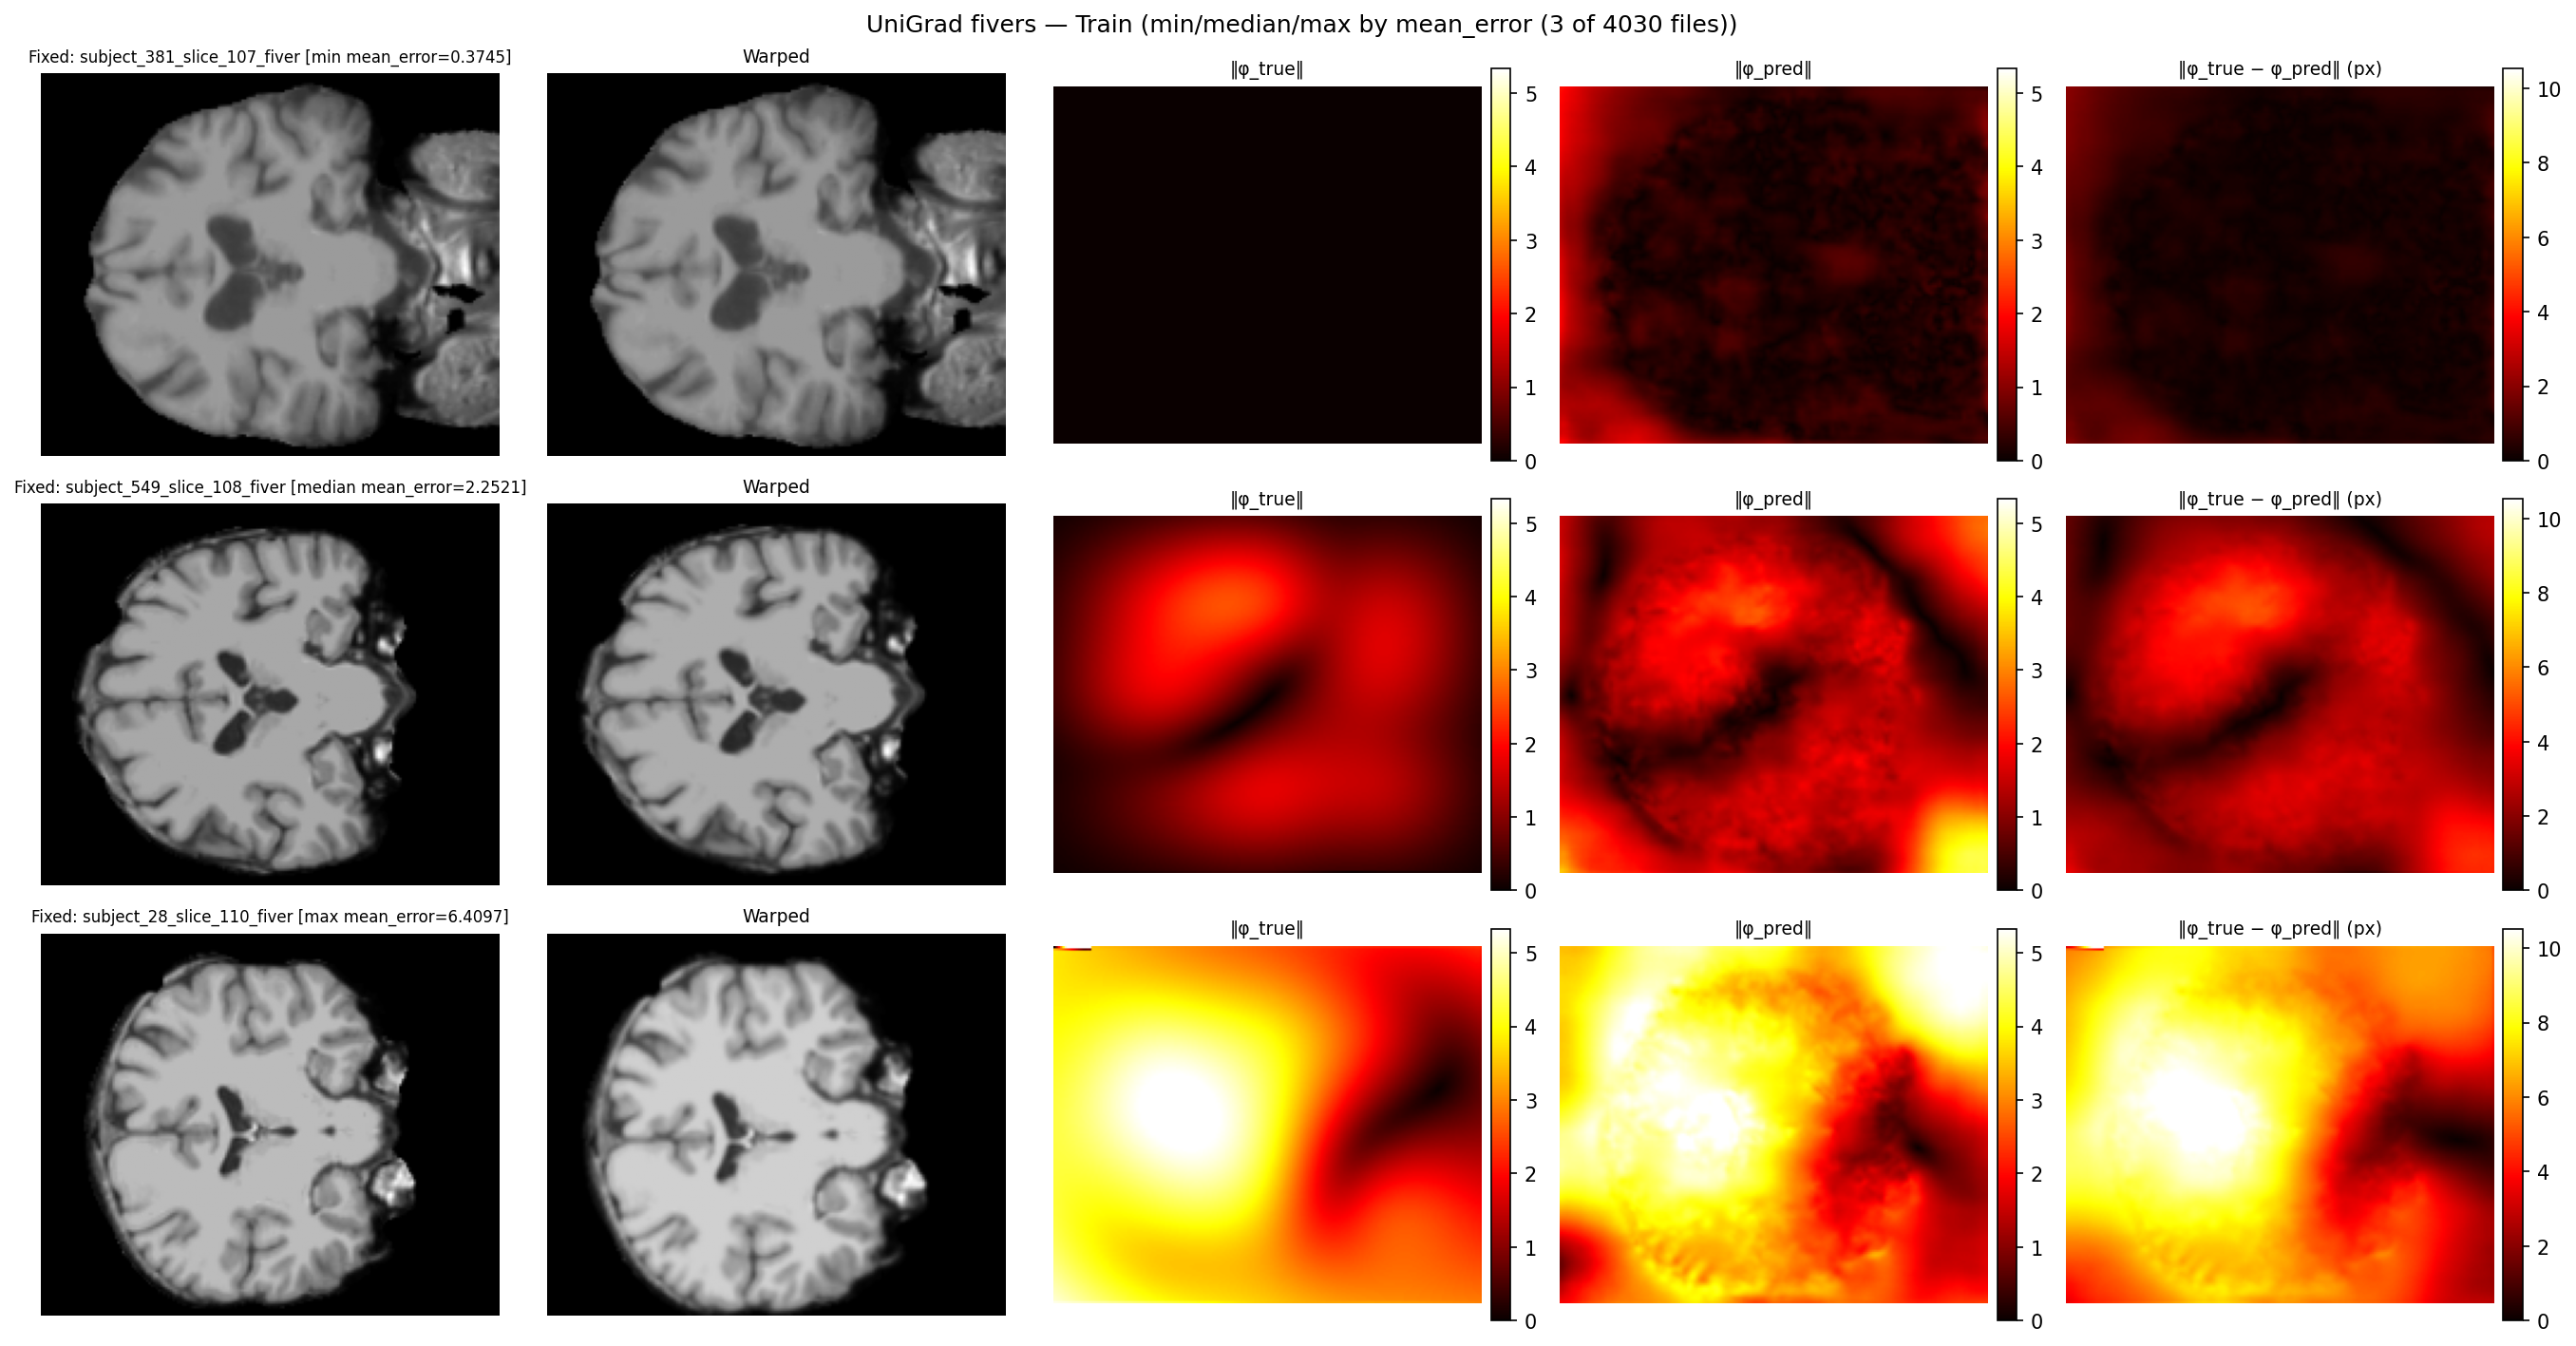
\includegraphics[width=0.95\linewidth]{assets/images/unigrad/ixi_unigrad_train_minmedmax.png}
  \caption{Train split fivers selected by deformation/error extremes (min/median/max) to inspect how predicted displacement magnitude relates to error magnitude.}
  \label{fig:unigrad_train_minmedmax}
\end{figure}

\paragraph{Why error-map supervision helps bypass the Correspondence Paradox.}
By using synthetic ground truth, Phase~2 provides a known pixelwise registration error map. This enables supervised learning of an ``uncertainty proxy'' $\,\hat{e}(u)\,$ using observable inputs and UniGradICON’s predicted deformation field, rather than relying on correspondence uncertainty to generate supervision signals.

\subsection{Phase 3: Supervised Error Map Training}
In Phase~3 we train a 2D U-Net to regress the scalar registration error map $e(u)$ produced in Phase~2.

\paragraph{Model inputs and output.}
Each training sample is built from the UniGrad fiver:
\begin{itemize}
  \item \emph{Input channels:} fixed image $I_{\text{fixed}}$, warped image $I_{\text{warped}}$, and $\phi_{\text{pred}}$ (two displacement components), concatenated into a 4-channel tensor.
  \item \emph{Output:} predicted error map $\hat{e}(u)$ (single channel).
\end{itemize}

In the default configuration, the network also applies per-slice robust intensity normalization to fixed/warped images before learning; $\phi_{\text{pred}}$ is scaled by a constant factor so that the regression operates on consistent pixel-displacement magnitudes.

\paragraph{Masked regression loss.}
Because boundaries can include transform artifacts and correspondences are less reliable near the periphery, training uses $\mathrm{valid\_mask}$ and computes the loss only over valid interior pixels:
\[
  \mathcal{L}_{\text{mse}}
  = \frac{1}{|\Omega_{\text{valid}}|}\sum_{u\in \Omega_{\text{valid}}}\left(\hat{e}(u)-e(u)\right)^2.
\]
This masked loss is implemented as a masked MSE averaged over valid pixels.

\paragraph{Optional boundary smoothness regularization.}
To reduce spurious oscillations near the transition between valid and invalid regions, an optional smoothness term can be added. The regularizer applies a gradient-based penalty to the prediction along edges where supervision is absent (i.e., at invalid regions), controlled by a hyperparameter $\texttt{smooth\_weight}$.

\paragraph{Optimization and checkpoint selection.}
Training uses AdamW with configurable hyperparameters (learning rate, weight decay) and validates after each epoch. We select the best checkpoint by the minimum validation masked MSE, producing a single final model used for evaluation.

\paragraph{Qualitative evaluation and error regime analysis.}
After training, we evaluate qualitative performance by selecting representative fivers from both the Test and Atlas splits. Two selection modes are used:
\begin{itemize}
  \item \emph{Random selection:} pick $N$ random samples from the split.
  \item \emph{Min/median/max selection:} rank samples by a scalar computed as the \emph{mean} error map over the slice. When available, the mean is masked by $\mathrm{valid\_mask}$. We then plot the min/median/max ranked samples to inspect behavior across low- and high-error regimes.
\end{itemize}

This design enables a compact visual analysis of how the predicted displacement magnitude $\|\phi_{\text{pred}}\|$ and the predicted scalar error map $\hat{e}(u)$ evolve across increasing ground-truth error.

\subsection{Summary Table: What Each Phase Produces}
\begin{table}[t]
  \centering
  \begin{tabular}{p{0.28\linewidth} p{0.67\linewidth}}
    \hline
    \textbf{Phase} & \textbf{Main output (data/artefacts)} \\
    \hline
    I. Ground Truth Generation &
    Synthetic $(I_{\text{fixed}}, I_{\text{warped}}, \phi_{\text{true}})$ triplets with
    $\mathrm{valid\_mask}$ and QC flags; deformation magnitude statistics are constrained via QC. \\
    \hline
    II. Error Map Generation &
    UniGradICON-derived $\phi_{\text{pred}}$ and residual displacement $\phi_{\text{diff}}$, producing the supervised scalar error map
    $e(u)=\|\phi_{\text{true}}(u)-\phi_{\text{pred}}(u)\|_2$ and propagating $\mathrm{valid\_mask}$ and QC flags. \\
    \hline
    III. Supervised Training &
    A U-Net regression model trained on masked MSE (and optional boundary smoothness) to predict $\hat{e}(u)$, with a best checkpoint selected by validation masked MSE. \\
    \hline
  \end{tabular}
  \caption{Summary of the three-stage pipeline and the primary supervision artefacts produced at each stage.}
  \label{tab:pipeline_outputs}
\end{table}


% Figure paths assume the main document's working directory contains assets/ as a sibling (adjust if needed).

\section{4. Methodology: The Three-Stage Workflow}
To investigate the connection between registration error and uncertainty, we built a modular pipeline designed to bypass the Correspondence Paradox. Instead of attempting to infer uncertainty directly from unknown correspondences, we generate synthetic deformations with known ground truth and then train a supervised regression model to predict the resulting registration error map.

Our pipeline has three distinct phases: (I) Ground Truth Data Generation, (II) Registration Error Map Generation, and (III) Supervised Error Map Training.

\subsection{Phase 1: Ground Truth Generation}
In Phase~1 we generate synthetic 2D registration triplets $(I_{\text{fixed}}, I_{\text{warped}}, \phi_{\text{true}})$ from raw IXI slices. Each synthetic sample is produced by applying a random affine deformation followed by a random elastic deformation to the slice geometry. The ground-truth displacement field is computed explicitly from the transformed sampling grid, enabling pixelwise supervision in later stages.

\paragraph{Random deformation and deformation field.}
Let $g_{\text{identity}}(u)$ denote the identity sampling grid at pixel location $u$, and let $g_{\text{transformed}}(u)$ be the sampling grid after applying the composed transforms. The synthetic displacement field is defined as
\[
  \phi_{\text{true}}(u) = g_{\text{transformed}}(u) - g_{\text{identity}}(u),
]
and the corresponding warped image $I_{\text{warped}}$ is obtained by the same transform used to compute $\phi_{\text{true}}$. The pipeline also defines an interior supervision region by excluding a boundary margin of $10$ pixels, producing a binary $\mathrm{valid\_mask}$ used to focus training on reliable pixels.

\paragraph{Quality control (QC) and dataset stability.}
To avoid degenerate deformations, each candidate sample undergoes QC acceptance checks on deformation magnitude and on warped intensity statistics. Candidate samples are attempted up to a fixed number of times; if QC still fails, the sample can be saved with $\mathrm{qc\_passed}=false$ (useful for optional regeneration/cleanup).

Key acceptance constraints include:
\begin{itemize}
  \item Affine parameters are constrained by pre-defined ranges for scale, rotation, and translation in pixels.
  \item Elastic deformation is constrained via the number of control points, maximum displacement magnitude, and application probability.
  \item Rejection if $|\phi|$ exceeds configured thresholds either on the interior band or globally.
  \item Rejection if the warped image is overly dark (a minimum ratio constraint on mean intensity).
\end{itemize}

\paragraph{Ground truth triplets (visual inspection).}
Figure~\ref{fig:triplet_examples} shows representative synthetic triplets for the Train split: fixed image, warped image, and the deformation magnitude $\|\phi\|$ in pixels.

\begin{figure}[t]
  \centering
  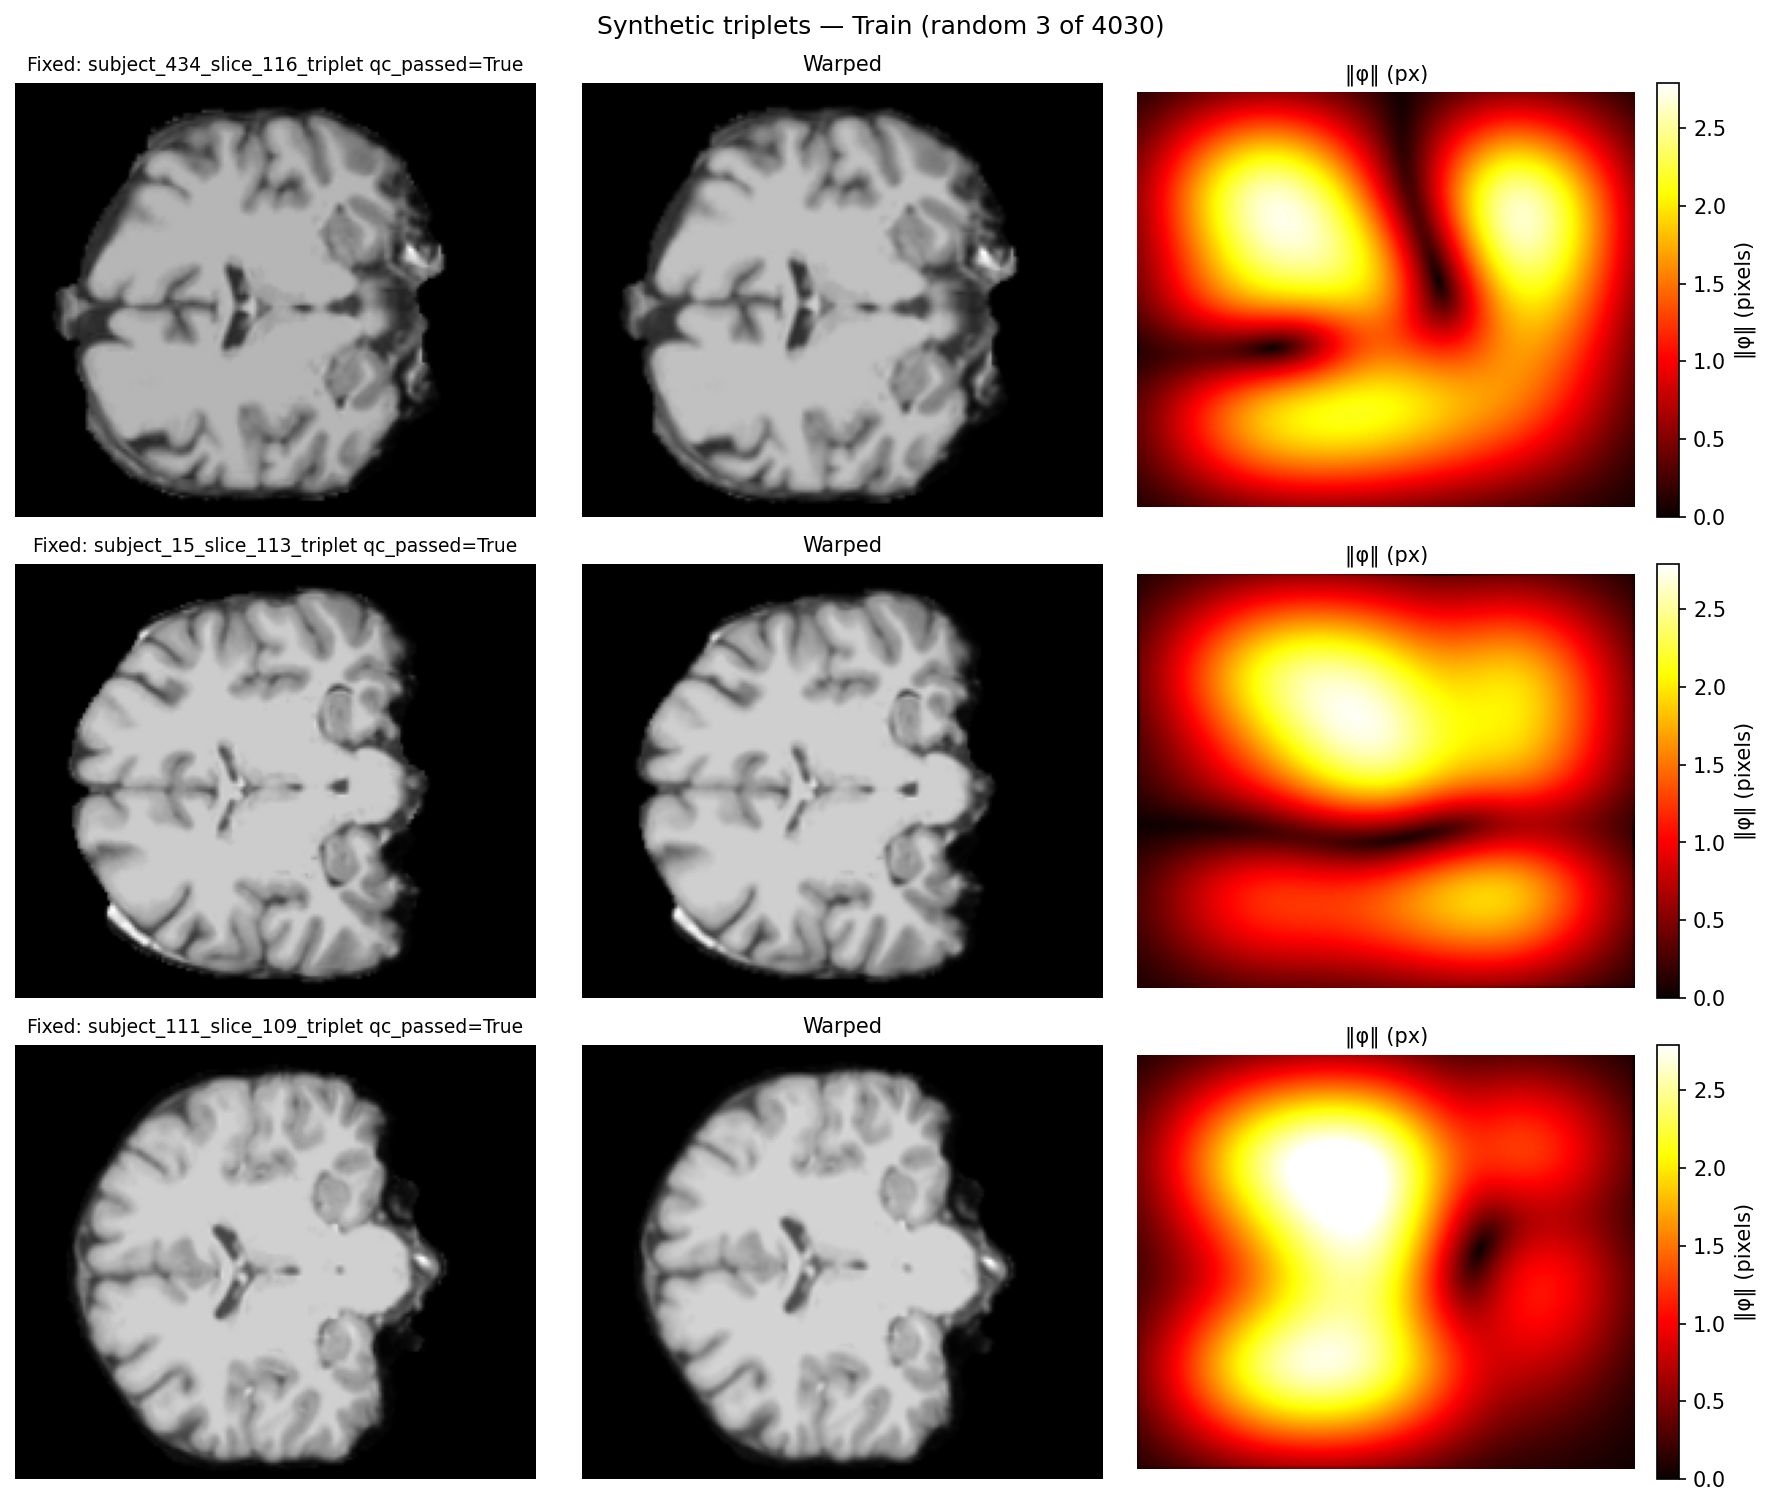
\includegraphics[width=0.95\linewidth]{assets/images/synthetic/ixi_synth_mtrain.png}
  \caption{Synthetic registration triplets generated in Phase~1 (fixed image, warped image, and deformation magnitude $\|\phi\|$).}
  \label{fig:triplet_examples}
\end{figure}

To support qualitative analysis across ``easy'' and ``hard'' deformation regimes, we additionally select min/median/max examples by a scalar $\phi$ statistic (default: mean deformation magnitude over the slice). Figure~\ref{fig:triplet_minmedmax} illustrates these representative extremes.

\begin{figure}[t]
  \centering
  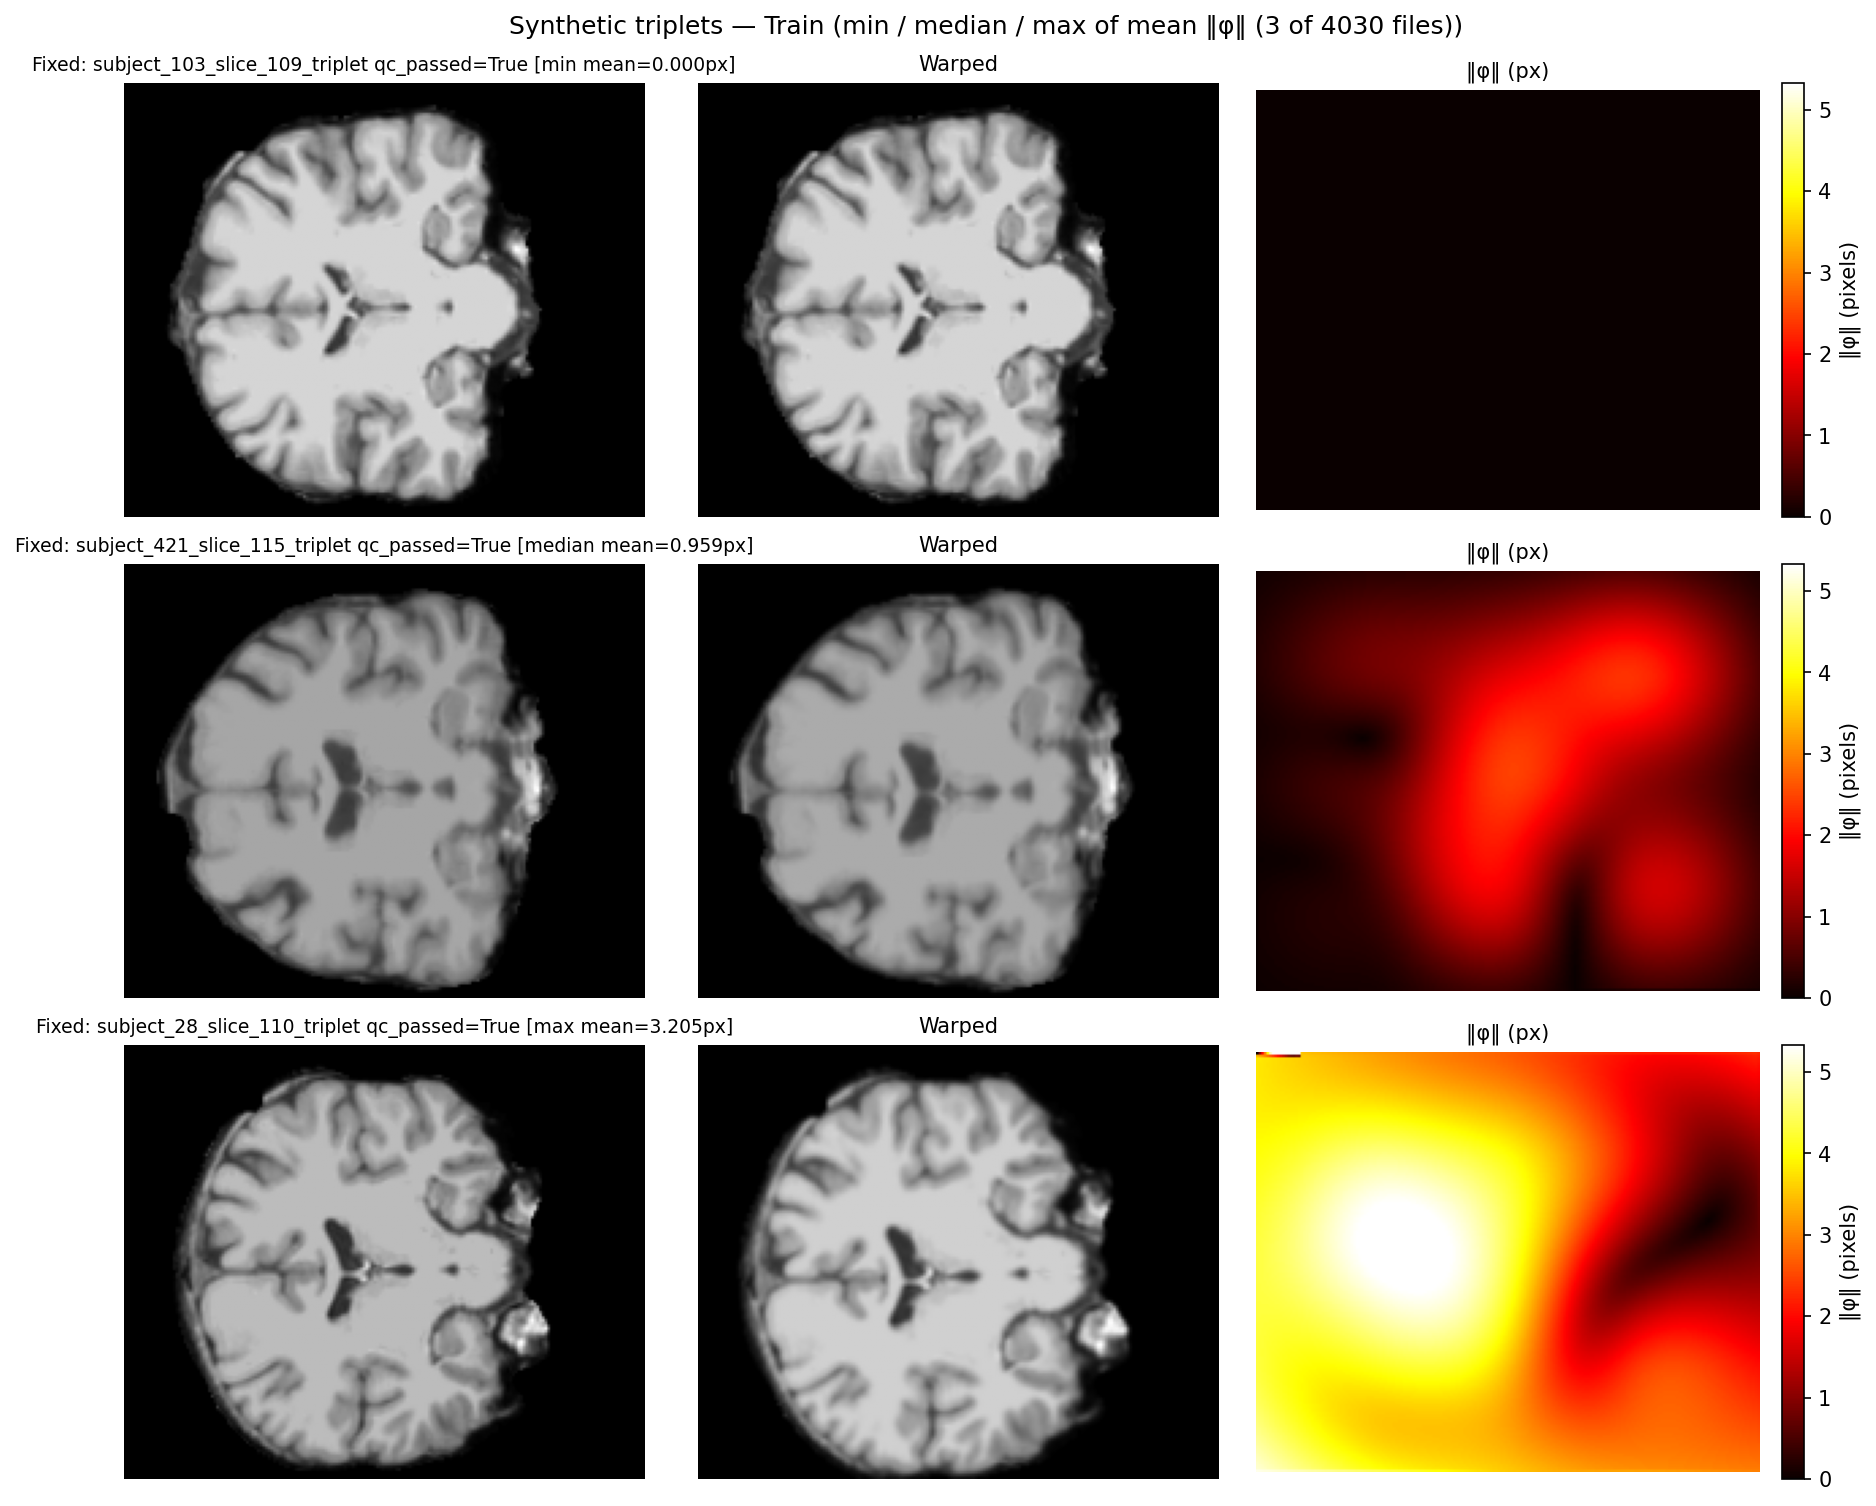
\includegraphics[width=0.95\linewidth]{assets/images/synthetic/ixi_synth_mtrain_minmedmax.png}
  \caption{Min/median/max synthetic triplets by deformation magnitude $\|\phi\|$ for the Train split.}
  \label{fig:triplet_minmedmax}
\end{figure}

\subsection{Phase 2: Registration Error Map Generation}
Phase~2 converts synthetic triplets into supervised scalar error maps by running UniGradICON to predict a deformation field and comparing it with the known synthetic ground truth.

\paragraph{UniGradICON fiver generation.}
For each triplet in each split (Train/Val/Test/Atlas), we:
\begin{itemize}
  \item Run UniGradICON to infer the deformation in the ICON coordinate system.
  \item Convert the predicted deformation back to the original 2D pixel grid to obtain $\phi_{\text{pred}}$ in pixel units.
  \item Compute the residual displacement $\phi_{\text{diff}}=\phi_{\text{true}}-\phi_{\text{pred}}$.
  \item Produce a scalar error map
  \[
    e(u) = \|\phi_{\text{true}}(u) - \phi_{\text{pred}}(u)\|_2
         = \sqrt{\Delta\phi_x(u)^2 + \Delta\phi_y(u)^2}.
  \]
\end{itemize}

The output fiver files ($\ast$$_\mathrm{fiver}$.npz) store, for each pixel, the fixed/warped images, $\phi_{\text{true}}$, $\phi_{\text{pred}}$, $\phi_{\text{diff}}$, and the scalar error map $e(u)$. Importantly, they also store $\mathrm{valid\_mask}$ and the QC flag propagated from Phase~1, enabling masked training later.

\paragraph{Phase~2 visualization.}
Figures~\ref{fig:unigrad_train} and \ref{fig:unigrad_train_minmedmax} show the UniGradICON-derived quantities for representative Train samples, including $\|\phi_{\text{true}}\|$, $\|\phi_{\text{pred}}\|$, and the scalar error map $\|\phi_{\text{true}}-\phi_{\text{pred}}\|$.

\begin{figure}[t]
  \centering
  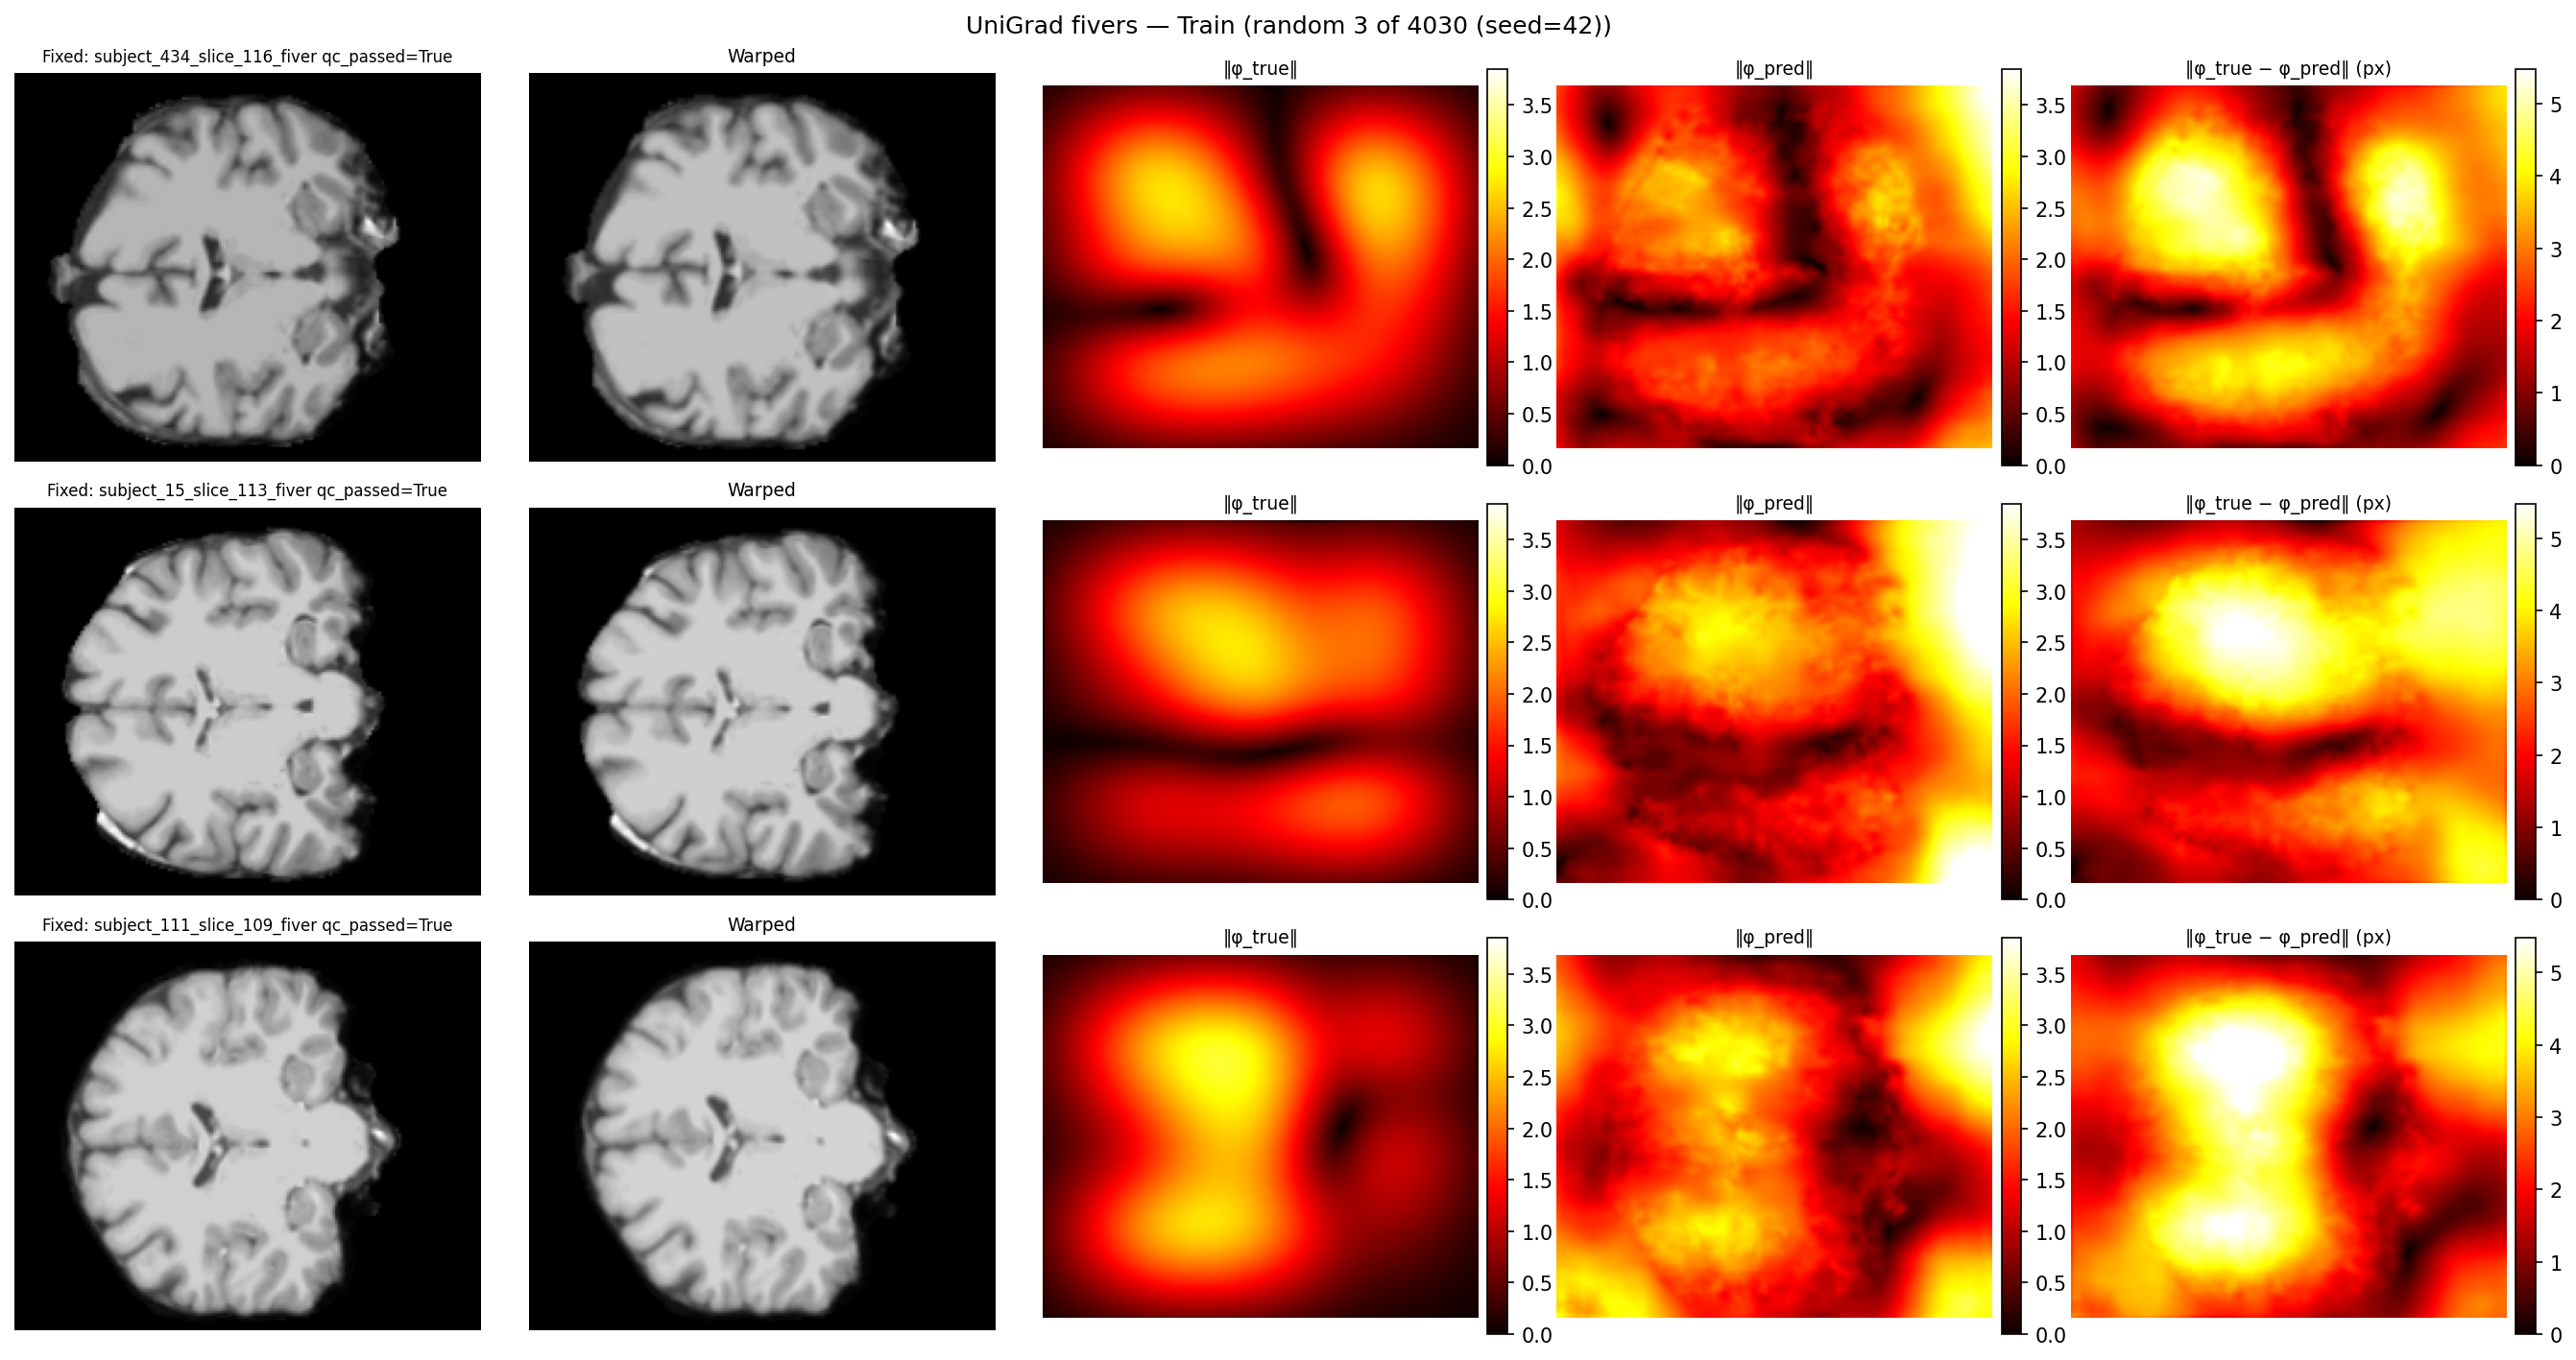
\includegraphics[width=0.95\linewidth]{assets/images/unigrad/ixi_unigrad_train.png}
  \caption{UniGradICON fiver visualization in Phase~2 for the Train split (including $\|\phi_{\text{true}}\|$, $\|\phi_{\text{pred}}\|$, and the scalar error map).}
  \label{fig:unigrad_train}
\end{figure}

\begin{figure}[t]
  \centering
  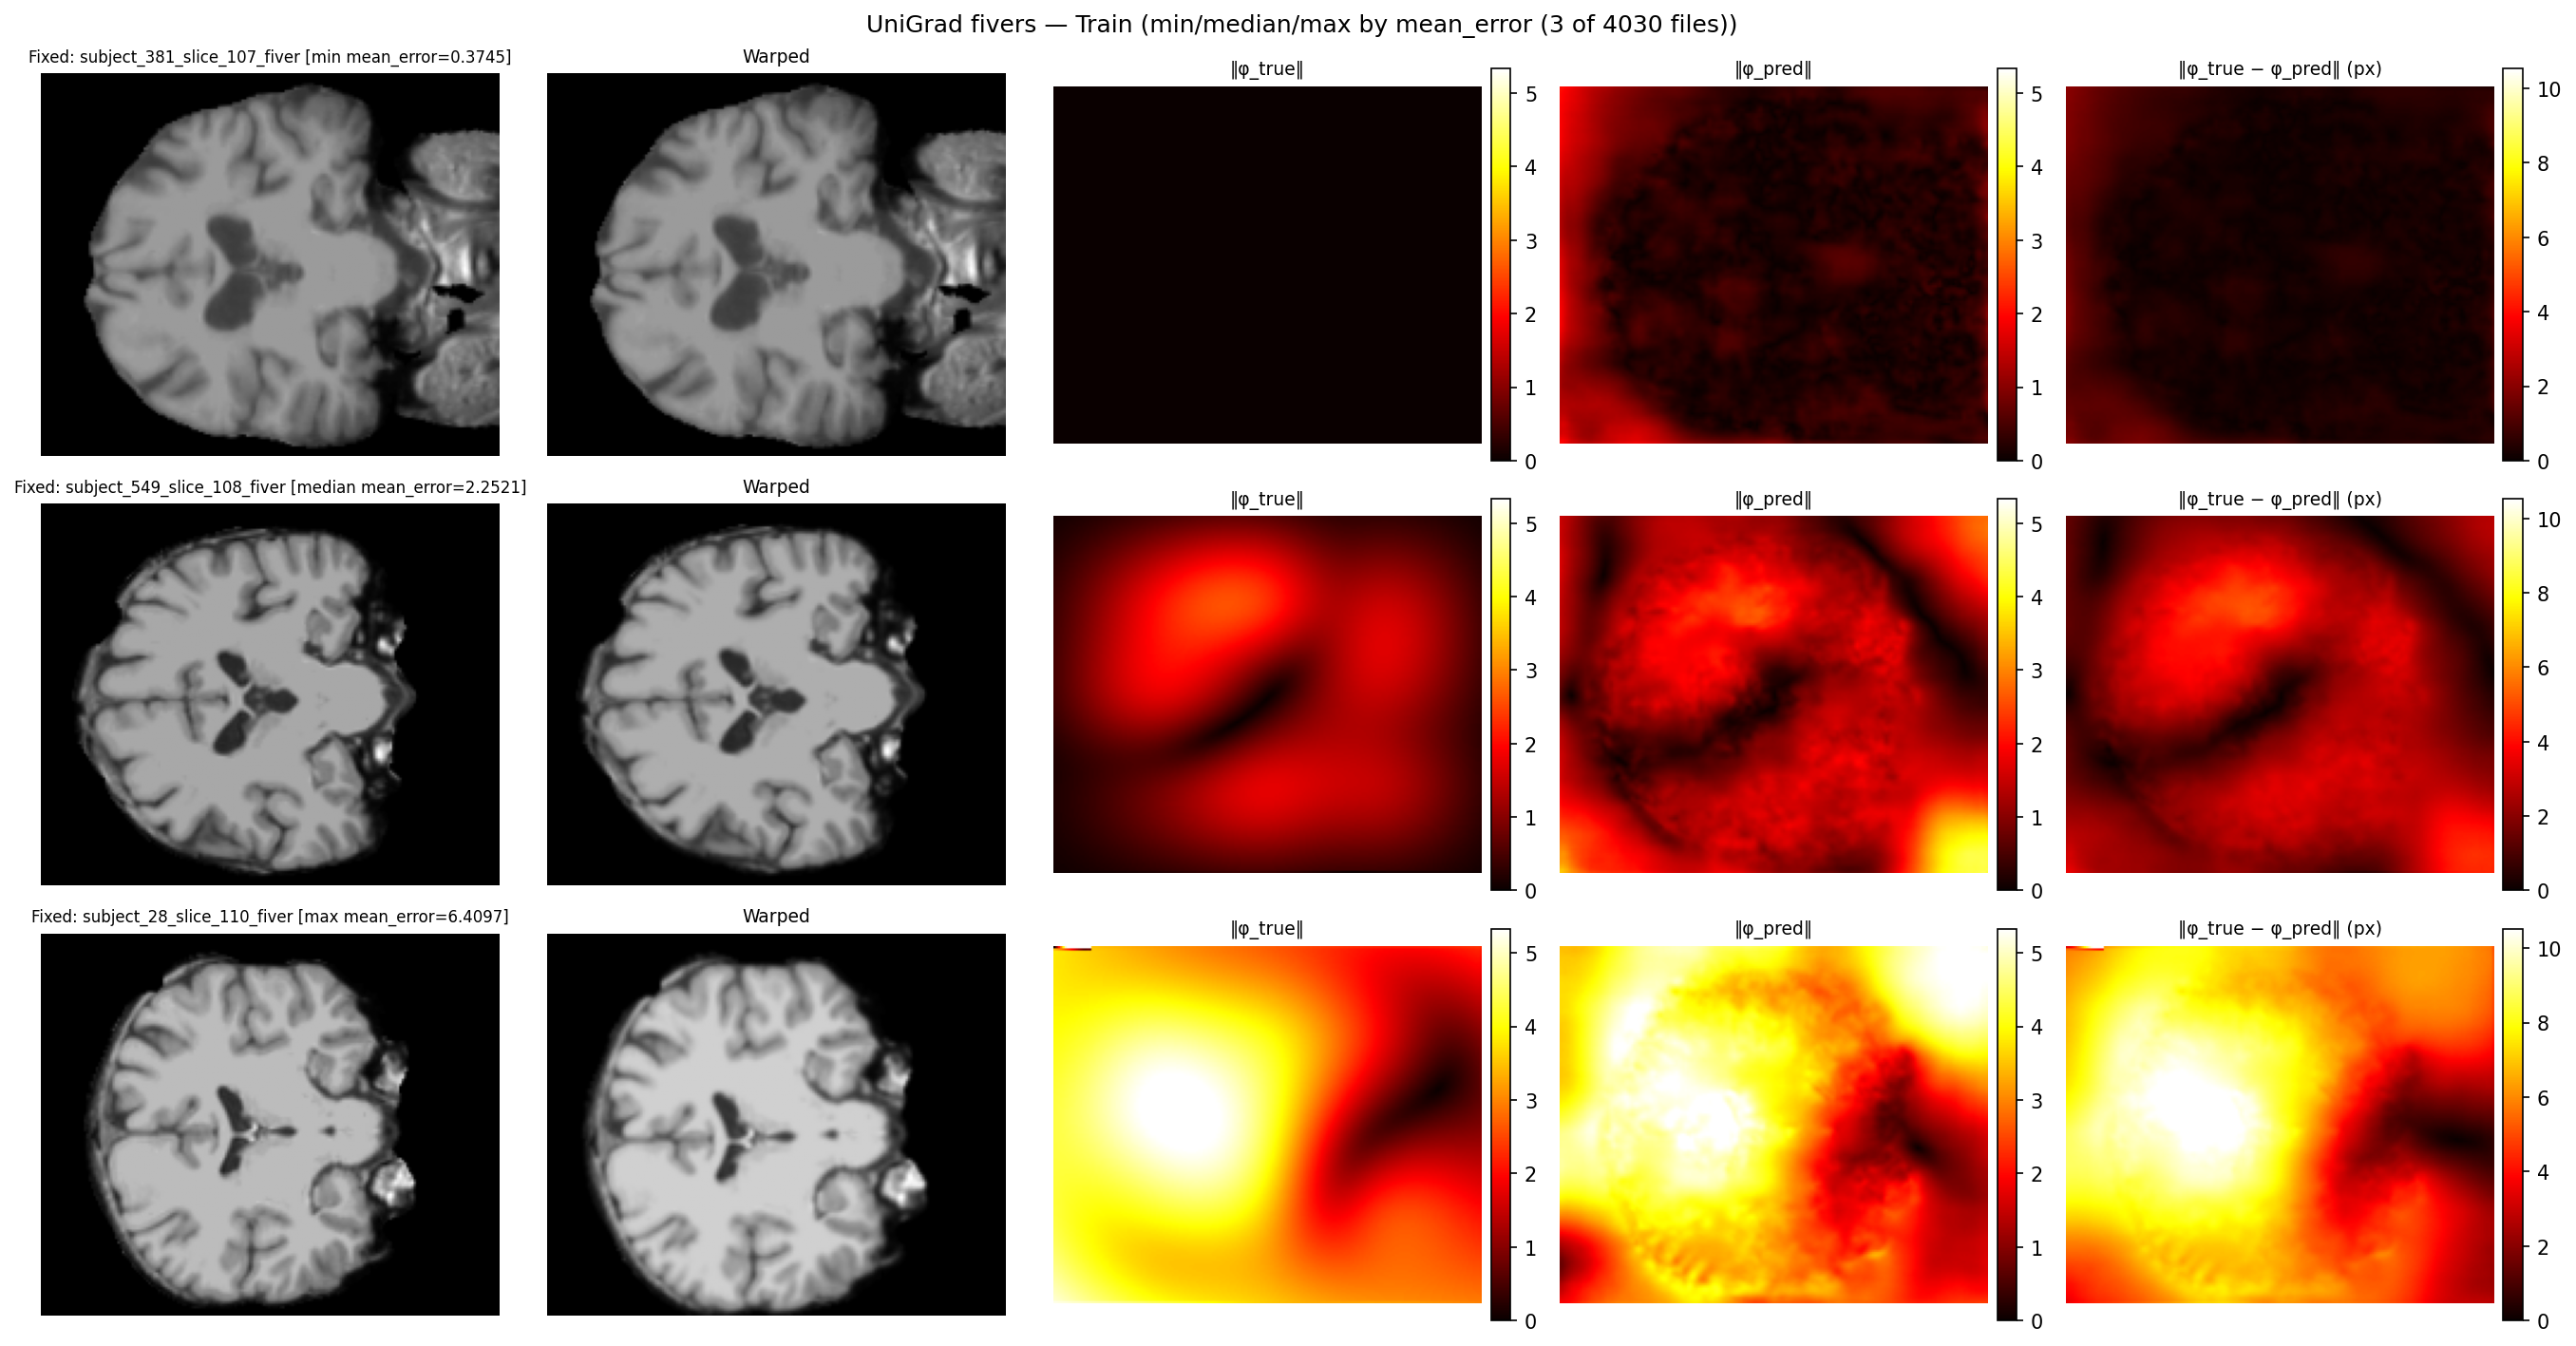
\includegraphics[width=0.95\linewidth]{assets/images/unigrad/ixi_unigrad_train_minmedmax.png}
  \caption{Train split fivers selected by deformation/error extremes (min/median/max) to inspect how predicted displacement magnitude relates to error magnitude.}
  \label{fig:unigrad_train_minmedmax}
\end{figure}

\paragraph{Why error-map supervision helps bypass the Correspondence Paradox.}
By using synthetic ground truth, Phase~2 provides a known pixelwise registration error map. This enables supervised learning of an ``uncertainty proxy'' $\,\hat{e}(u)\,$ using observable inputs and UniGradICON’s predicted deformation field, rather than relying on correspondence uncertainty to generate supervision signals.

\subsection{Phase 3: Supervised Error Map Training}
In Phase~3 we train a 2D U-Net to regress the scalar registration error map $e(u)$ produced in Phase~2.

\paragraph{Model inputs and output.}
Each training sample is built from the UniGrad fiver:
\begin{itemize}
  \item \emph{Input channels:} fixed image $I_{\text{fixed}}$, warped image $I_{\text{warped}}$, and $\phi_{\text{pred}}$ (two displacement components), concatenated into a 4-channel tensor.
  \item \emph{Output:} predicted error map $\hat{e}(u)$ (single channel).
\end{itemize}

In the default configuration, the network also applies per-slice robust intensity normalization to fixed/warped images before learning; $\phi_{\text{pred}}$ is scaled by a constant factor so that the regression operates on consistent pixel-displacement magnitudes.

\paragraph{Masked regression loss.}
Because boundaries can include transform artifacts and correspondences are less reliable near the periphery, training uses $\mathrm{valid\_mask}$ and computes the loss only over valid interior pixels:
\[
  \mathcal{L}_{\text{mse}}
  = \frac{1}{|\Omega_{\text{valid}}|}\sum_{u\in \Omega_{\text{valid}}}\left(\hat{e}(u)-e(u)\right)^2.
\]
This masked loss is implemented as a masked MSE averaged over valid pixels.

\paragraph{Optional boundary smoothness regularization.}
To reduce spurious oscillations near the transition between valid and invalid regions, an optional smoothness term can be added. The regularizer applies a gradient-based penalty to the prediction along edges where supervision is absent (i.e., at invalid regions), controlled by a hyperparameter $\texttt{smooth\_weight}$.

\paragraph{Optimization and checkpoint selection.}
Training uses AdamW with configurable hyperparameters (learning rate, weight decay) and validates after each epoch. We select the best checkpoint by the minimum validation masked MSE, producing a single final model used for evaluation.

\paragraph{Qualitative evaluation and error regime analysis.}
After training, we evaluate qualitative performance by selecting representative fivers from both the Test and Atlas splits. Two selection modes are used:
\begin{itemize}
  \item \emph{Random selection:} pick $N$ random samples from the split.
  \item \emph{Min/median/max selection:} rank samples by a scalar computed as the \emph{mean} error map over the slice. When available, the mean is masked by $\mathrm{valid\_mask}$. We then plot the min/median/max ranked samples to inspect behavior across low- and high-error regimes.
\end{itemize}

This design enables a compact visual analysis of how the predicted displacement magnitude $\|\phi_{\text{pred}}\|$ and the predicted scalar error map $\hat{e}(u)$ evolve across increasing ground-truth error.

\subsection{Summary Table: What Each Phase Produces}
\begin{table}[t]
  \centering
  \begin{tabular}{p{0.28\linewidth} p{0.67\linewidth}}
    \hline
    \textbf{Phase} & \textbf{Main output (data/artefacts)} \\
    \hline
    I. Ground Truth Generation &
    Synthetic $(I_{\text{fixed}}, I_{\text{warped}}, \phi_{\text{true}})$ triplets with
    $\mathrm{valid\_mask}$ and QC flags; deformation magnitude statistics are constrained via QC. \\
    \hline
    II. Error Map Generation &
    UniGradICON-derived $\phi_{\text{pred}}$ and residual displacement $\phi_{\text{diff}}$, producing the supervised scalar error map
    $e(u)=\|\phi_{\text{true}}(u)-\phi_{\text{pred}}(u)\|_2$ and propagating $\mathrm{valid\_mask}$ and QC flags. \\
    \hline
    III. Supervised Training &
    A U-Net regression model trained on masked MSE (and optional boundary smoothness) to predict $\hat{e}(u)$, with a best checkpoint selected by validation masked MSE. \\
    \hline
  \end{tabular}
  \caption{Summary of the three-stage pipeline and the primary supervision artefacts produced at each stage.}
  \label{tab:pipeline_outputs}
\end{table}


% Figure paths assume the main document's working directory contains assets/ as a sibling (adjust if needed).

\section{4. Methodology: The Three-Stage Workflow}
To investigate the connection between registration error and uncertainty, we built a modular pipeline designed to bypass the Correspondence Paradox. Instead of attempting to infer uncertainty directly from unknown correspondences, we generate synthetic deformations with known ground truth and then train a supervised regression model to predict the resulting registration error map.

Our pipeline has three distinct phases: (I) Ground Truth Data Generation, (II) Registration Error Map Generation, and (III) Supervised Error Map Training.

\subsection{Phase 1: Ground Truth Generation}
In Phase~1 we generate synthetic 2D registration triplets $(I_{\text{fixed}}, I_{\text{warped}}, \phi_{\text{true}})$ from raw IXI slices. Each synthetic sample is produced by applying a random affine deformation followed by a random elastic deformation to the slice geometry. The ground-truth displacement field is computed explicitly from the transformed sampling grid, enabling pixelwise supervision in later stages.

\paragraph{Random deformation and deformation field.}
Let $g_{\text{identity}}(u)$ denote the identity sampling grid at pixel location $u$, and let $g_{\text{transformed}}(u)$ be the sampling grid after applying the composed transforms. The synthetic displacement field is defined as
\[
  \phi_{\text{true}}(u) = g_{\text{transformed}}(u) - g_{\text{identity}}(u),
]
and the corresponding warped image $I_{\text{warped}}$ is obtained by the same transform used to compute $\phi_{\text{true}}$. The pipeline also defines an interior supervision region by excluding a boundary margin of $10$ pixels, producing a binary $\mathrm{valid\_mask}$ used to focus training on reliable pixels.

\paragraph{Quality control (QC) and dataset stability.}
To avoid degenerate deformations, each candidate sample undergoes QC acceptance checks on deformation magnitude and on warped intensity statistics. Candidate samples are attempted up to a fixed number of times; if QC still fails, the sample can be saved with $\mathrm{qc\_passed}=false$ (useful for optional regeneration/cleanup).

Key acceptance constraints include:
\begin{itemize}
  \item Affine parameters are constrained by pre-defined ranges for scale, rotation, and translation in pixels.
  \item Elastic deformation is constrained via the number of control points, maximum displacement magnitude, and application probability.
  \item Rejection if $|\phi|$ exceeds configured thresholds either on the interior band or globally.
  \item Rejection if the warped image is overly dark (a minimum ratio constraint on mean intensity).
\end{itemize}

\paragraph{Ground truth triplets (visual inspection).}
Figure~\ref{fig:triplet_examples} shows representative synthetic triplets for the Train split: fixed image, warped image, and the deformation magnitude $\|\phi\|$ in pixels.

\begin{figure}[t]
  \centering
  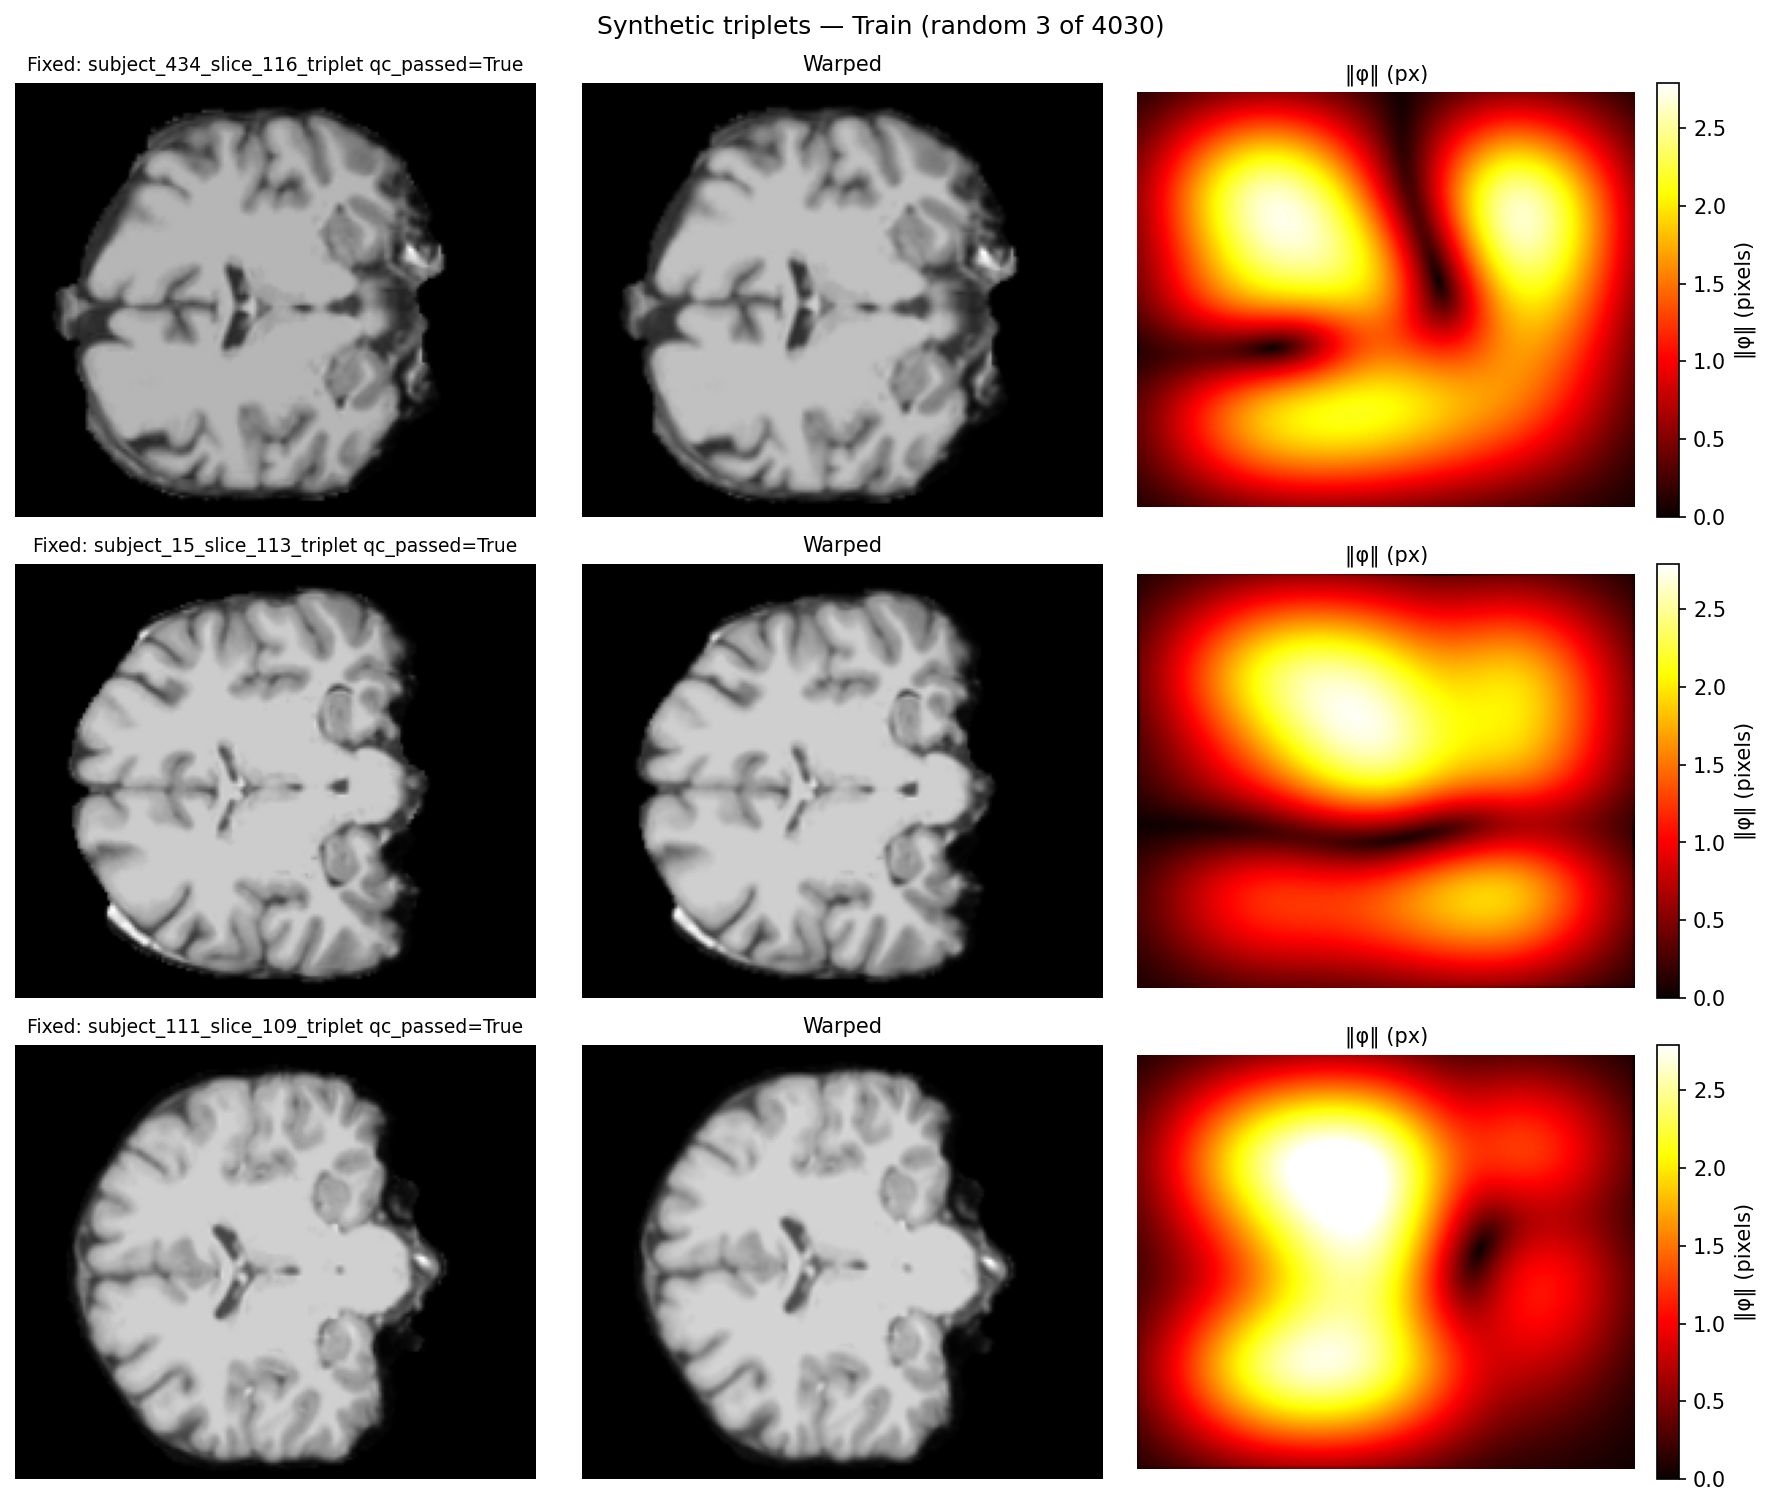
\includegraphics[width=0.95\linewidth]{assets/images/synthetic/ixi_synth_mtrain.png}
  \caption{Synthetic registration triplets generated in Phase~1 (fixed image, warped image, and deformation magnitude $\|\phi\|$).}
  \label{fig:triplet_examples}
\end{figure}

To support qualitative analysis across ``easy'' and ``hard'' deformation regimes, we additionally select min/median/max examples by a scalar $\phi$ statistic (default: mean deformation magnitude over the slice). Figure~\ref{fig:triplet_minmedmax} illustrates these representative extremes.

\begin{figure}[t]
  \centering
  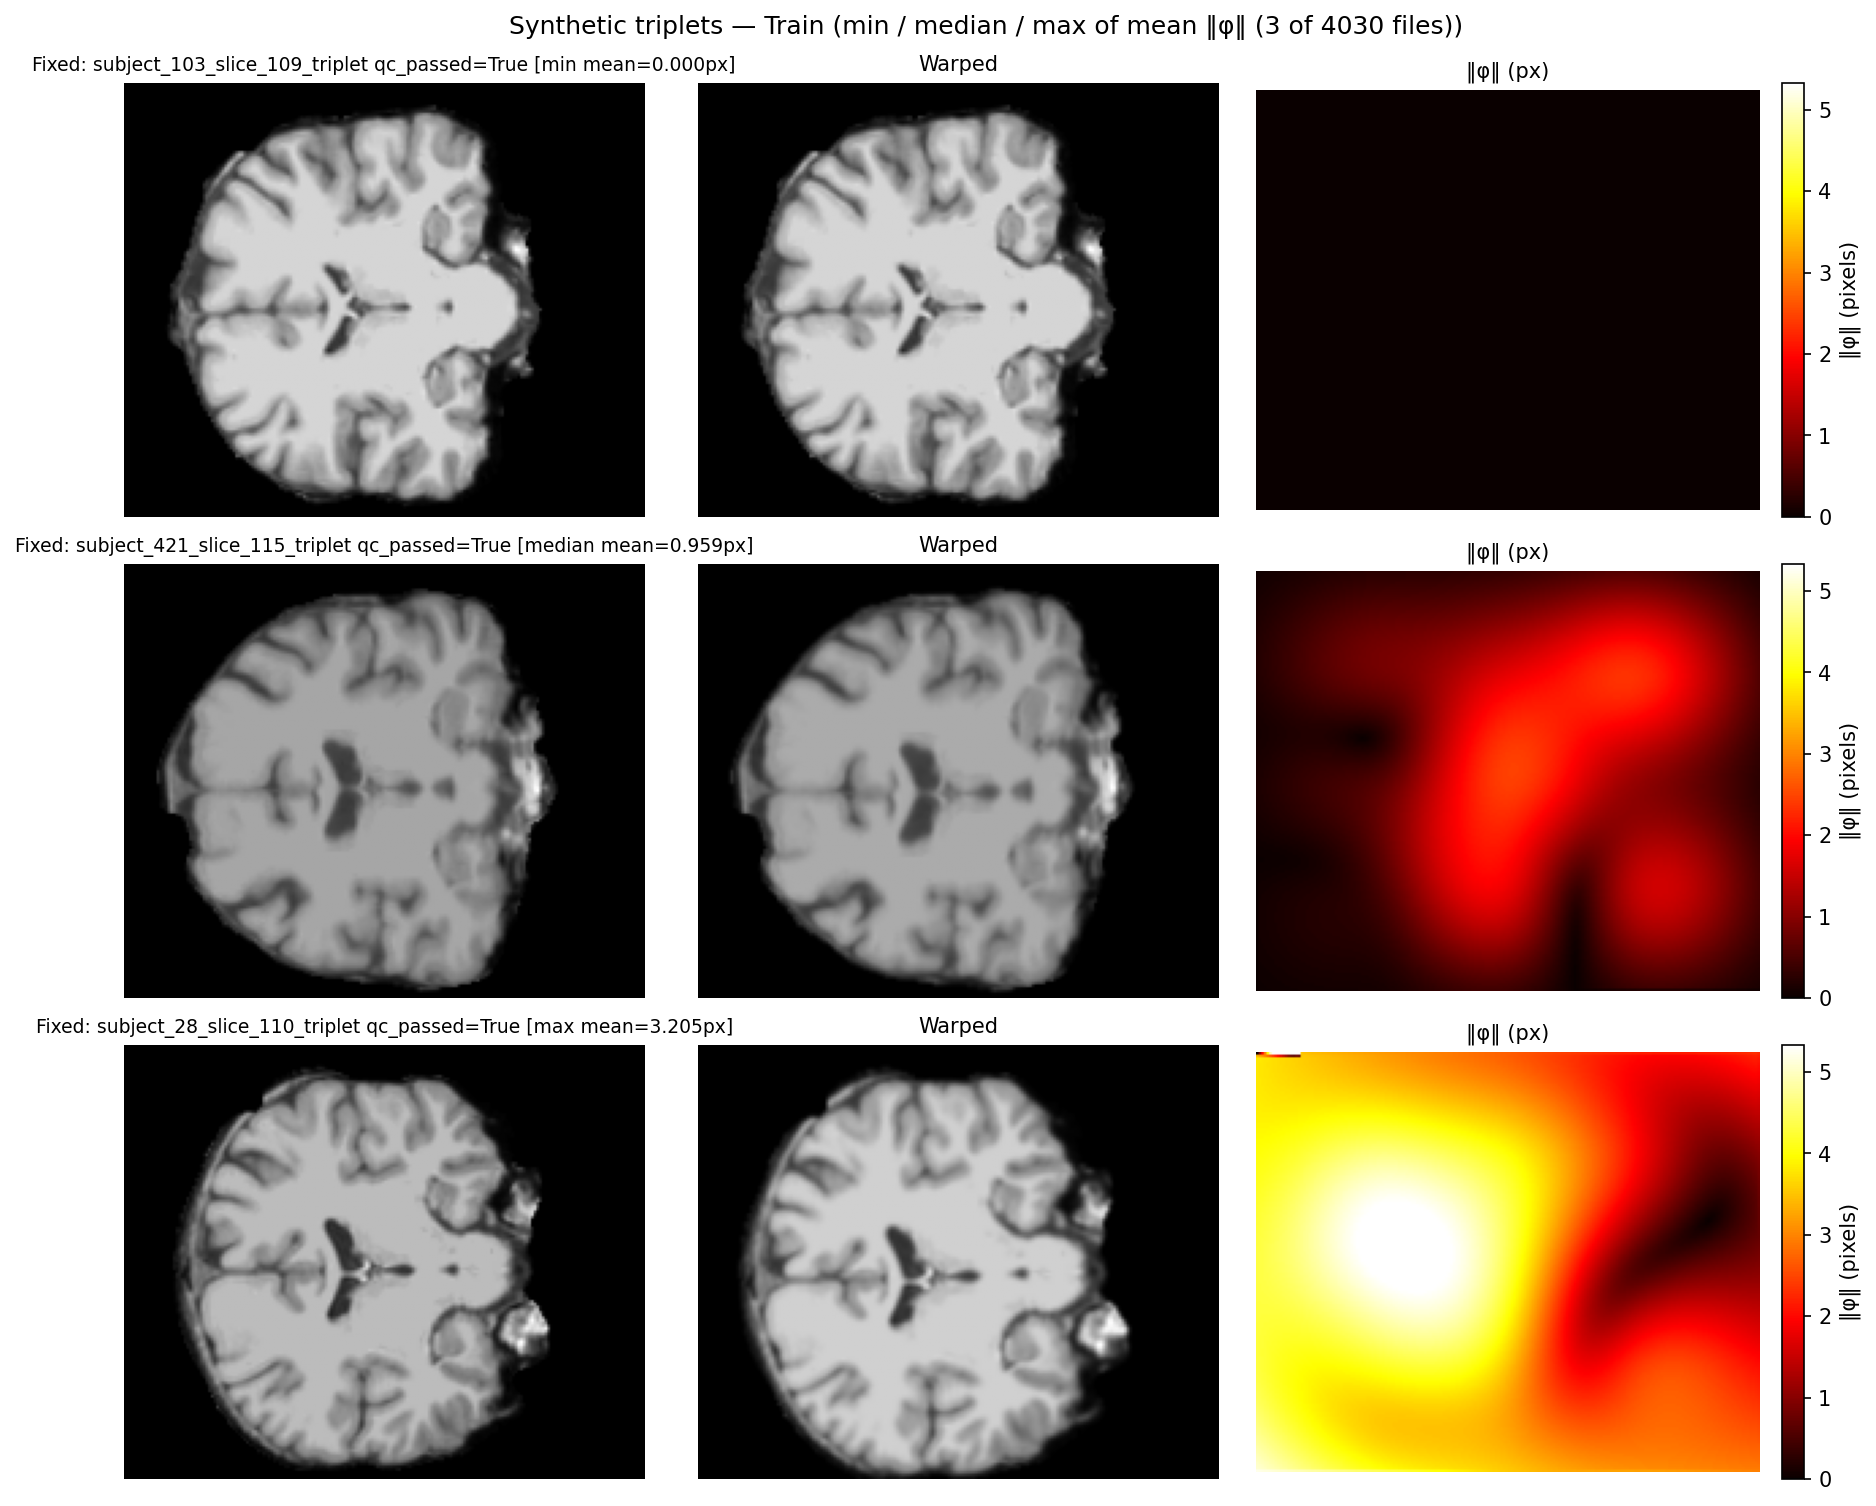
\includegraphics[width=0.95\linewidth]{assets/images/synthetic/ixi_synth_mtrain_minmedmax.png}
  \caption{Min/median/max synthetic triplets by deformation magnitude $\|\phi\|$ for the Train split.}
  \label{fig:triplet_minmedmax}
\end{figure}

\subsection{Phase 2: Registration Error Map Generation}
Phase~2 converts synthetic triplets into supervised scalar error maps by running UniGradICON to predict a deformation field and comparing it with the known synthetic ground truth.

\paragraph{UniGradICON fiver generation.}
For each triplet in each split (Train/Val/Test/Atlas), we:
\begin{itemize}
  \item Run UniGradICON to infer the deformation in the ICON coordinate system.
  \item Convert the predicted deformation back to the original 2D pixel grid to obtain $\phi_{\text{pred}}$ in pixel units.
  \item Compute the residual displacement $\phi_{\text{diff}}=\phi_{\text{true}}-\phi_{\text{pred}}$.
  \item Produce a scalar error map
  \[
    e(u) = \|\phi_{\text{true}}(u) - \phi_{\text{pred}}(u)\|_2
         = \sqrt{\Delta\phi_x(u)^2 + \Delta\phi_y(u)^2}.
  \]
\end{itemize}

The output fiver files ($\ast$$_\mathrm{fiver}$.npz) store, for each pixel, the fixed/warped images, $\phi_{\text{true}}$, $\phi_{\text{pred}}$, $\phi_{\text{diff}}$, and the scalar error map $e(u)$. Importantly, they also store $\mathrm{valid\_mask}$ and the QC flag propagated from Phase~1, enabling masked training later.

\paragraph{Phase~2 visualization.}
Figures~\ref{fig:unigrad_train} and \ref{fig:unigrad_train_minmedmax} show the UniGradICON-derived quantities for representative Train samples, including $\|\phi_{\text{true}}\|$, $\|\phi_{\text{pred}}\|$, and the scalar error map $\|\phi_{\text{true}}-\phi_{\text{pred}}\|$.

\begin{figure}[t]
  \centering
  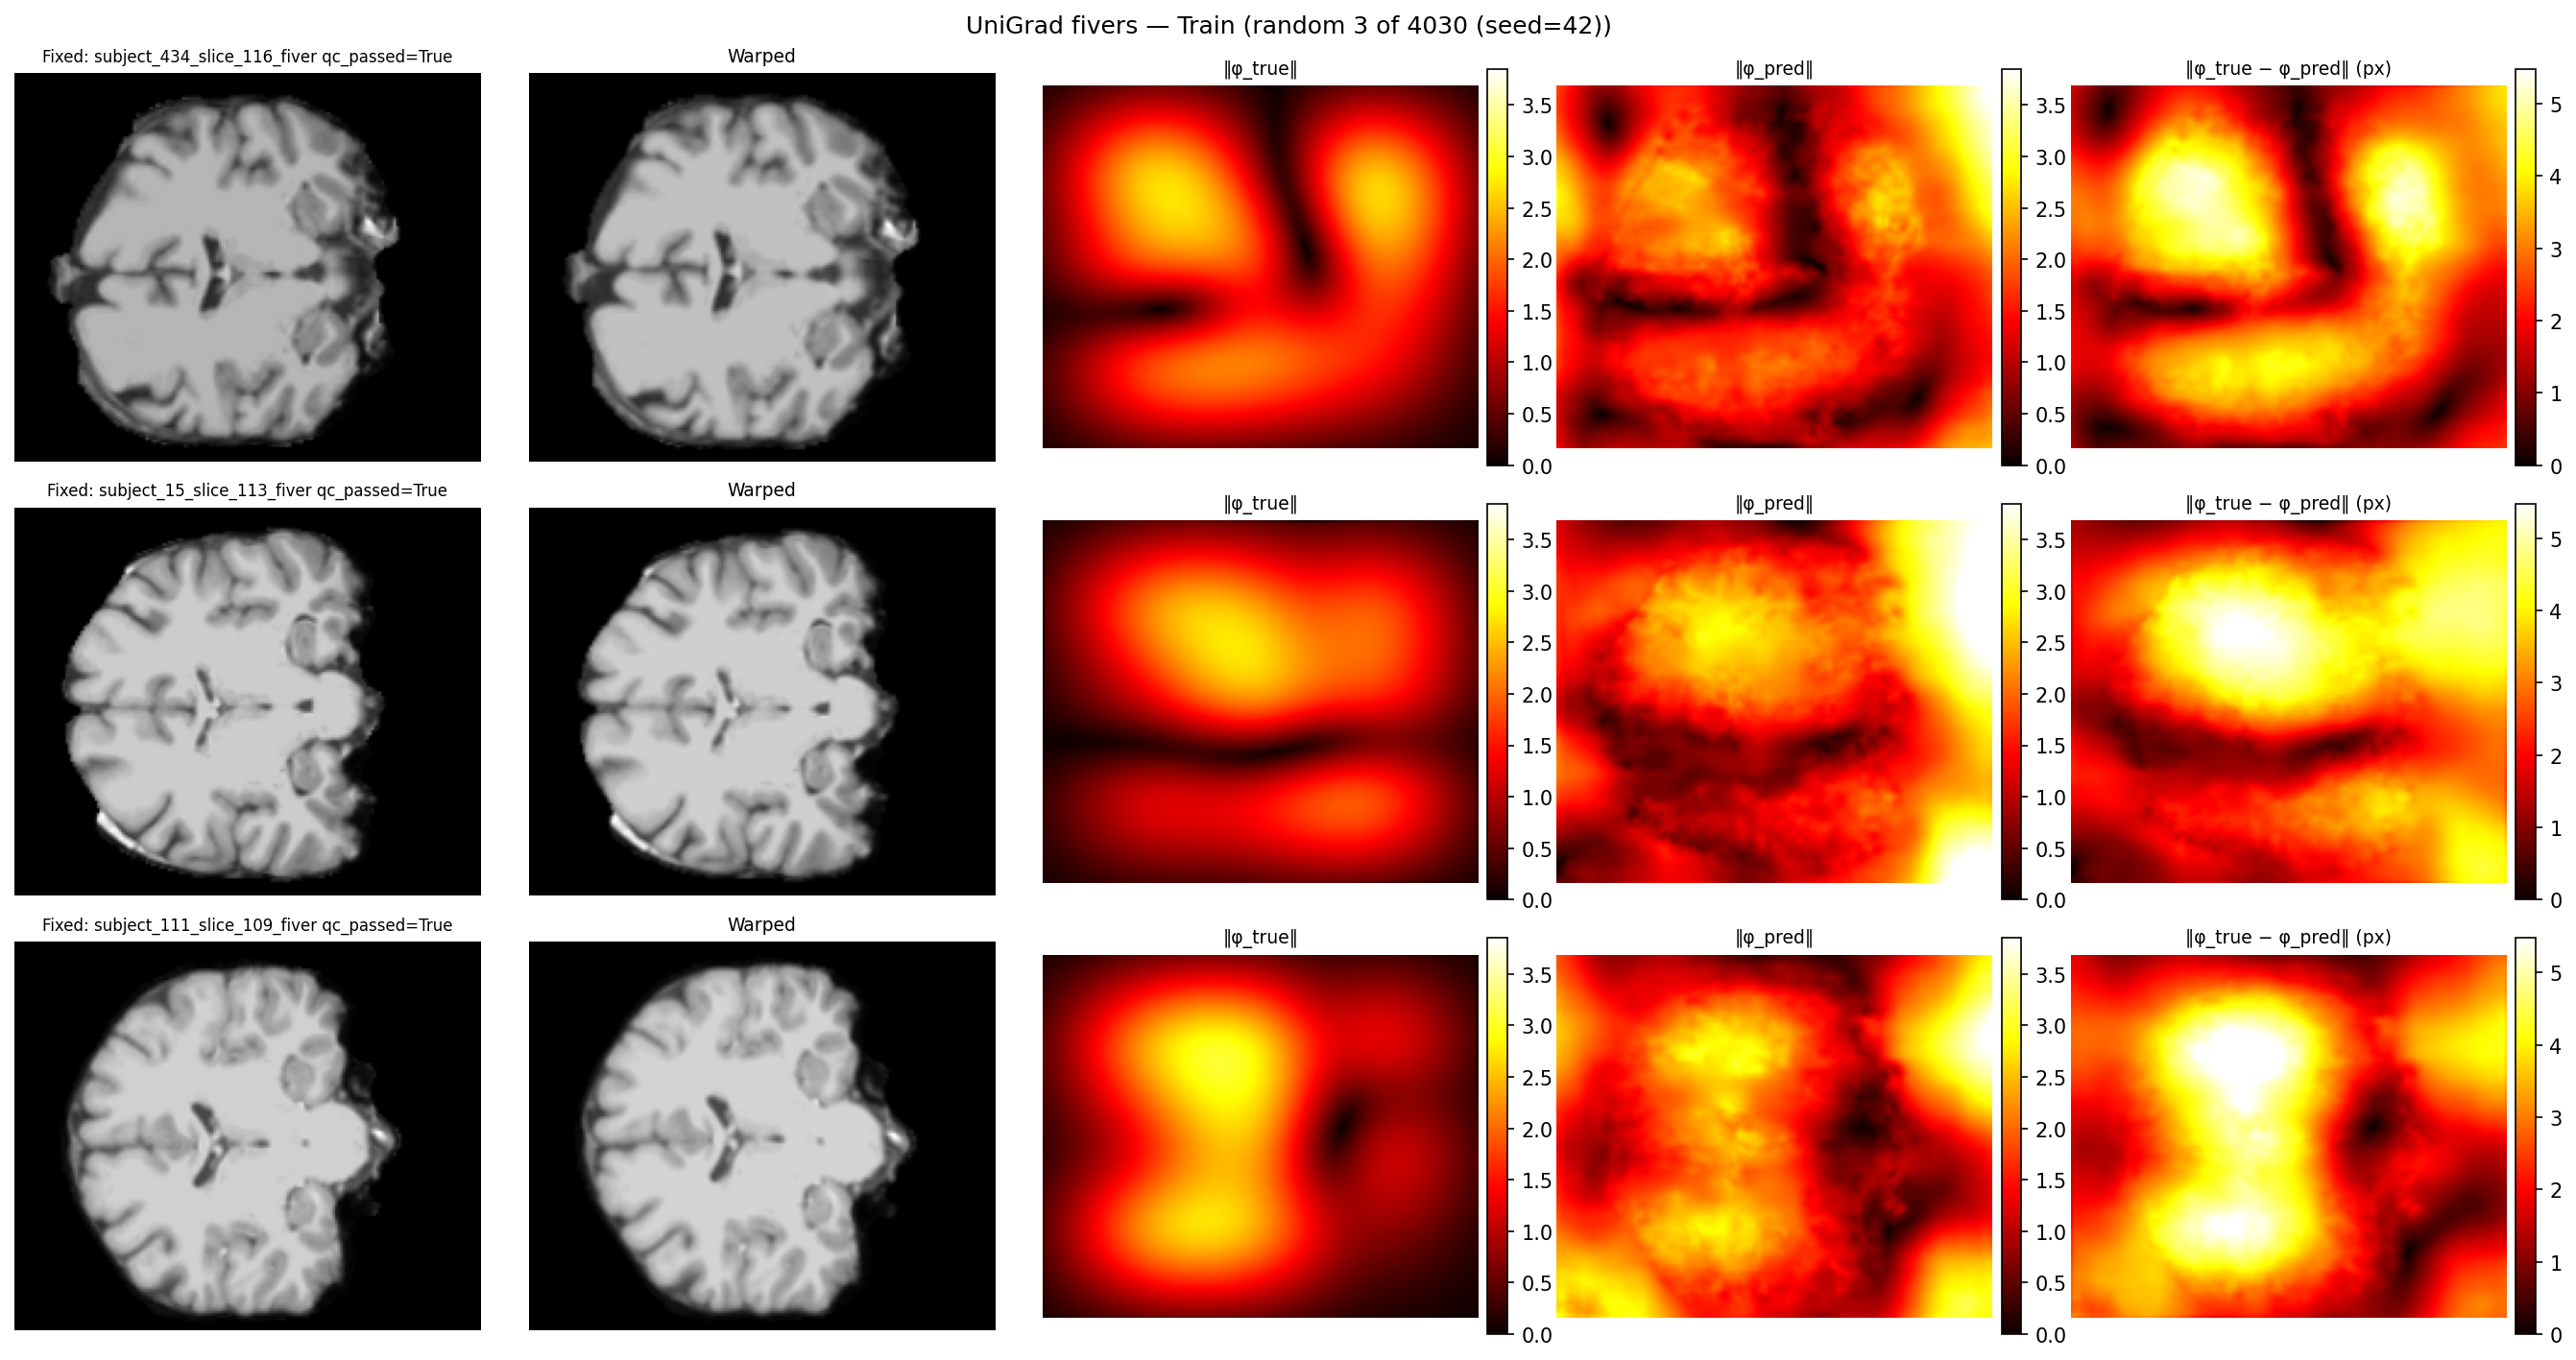
\includegraphics[width=0.95\linewidth]{assets/images/unigrad/ixi_unigrad_train.png}
  \caption{UniGradICON fiver visualization in Phase~2 for the Train split (including $\|\phi_{\text{true}}\|$, $\|\phi_{\text{pred}}\|$, and the scalar error map).}
  \label{fig:unigrad_train}
\end{figure}

\begin{figure}[t]
  \centering
  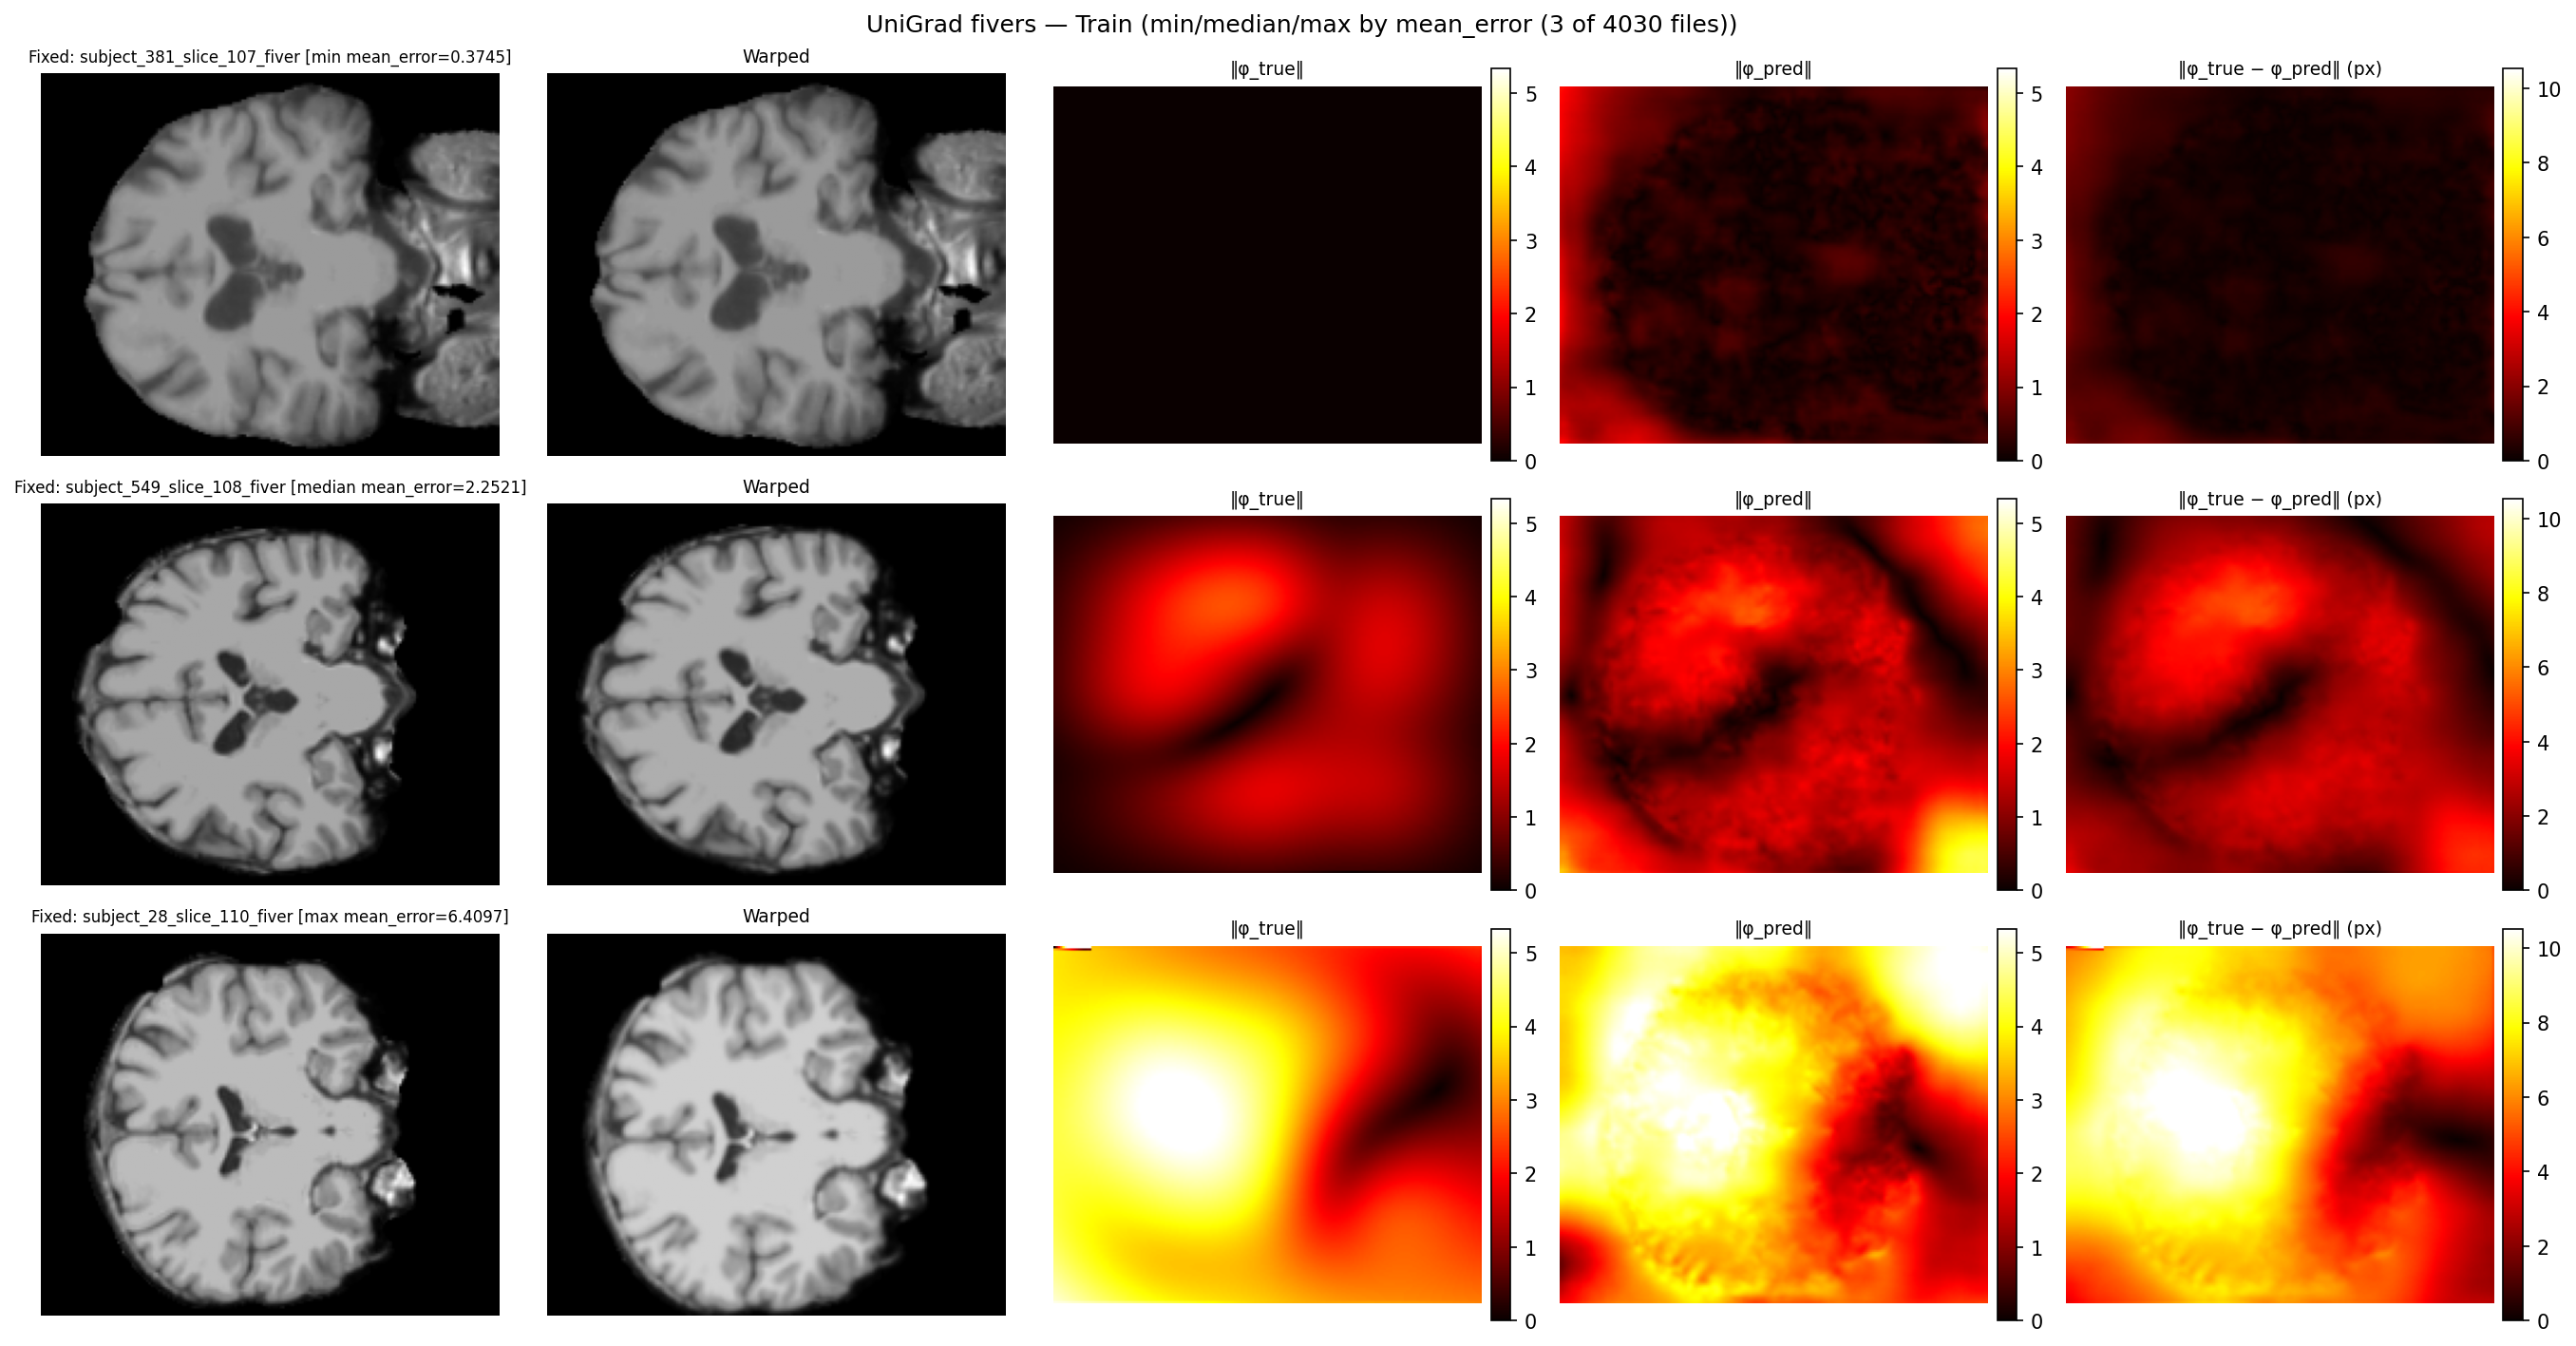
\includegraphics[width=0.95\linewidth]{assets/images/unigrad/ixi_unigrad_train_minmedmax.png}
  \caption{Train split fivers selected by deformation/error extremes (min/median/max) to inspect how predicted displacement magnitude relates to error magnitude.}
  \label{fig:unigrad_train_minmedmax}
\end{figure}

\paragraph{Why error-map supervision helps bypass the Correspondence Paradox.}
By using synthetic ground truth, Phase~2 provides a known pixelwise registration error map. This enables supervised learning of an ``uncertainty proxy'' $\,\hat{e}(u)\,$ using observable inputs and UniGradICON’s predicted deformation field, rather than relying on correspondence uncertainty to generate supervision signals.

\subsection{Phase 3: Supervised Error Map Training}
In Phase~3 we train a 2D U-Net to regress the scalar registration error map $e(u)$ produced in Phase~2.

\paragraph{Model inputs and output.}
Each training sample is built from the UniGrad fiver:
\begin{itemize}
  \item \emph{Input channels:} fixed image $I_{\text{fixed}}$, warped image $I_{\text{warped}}$, and $\phi_{\text{pred}}$ (two displacement components), concatenated into a 4-channel tensor.
  \item \emph{Output:} predicted error map $\hat{e}(u)$ (single channel).
\end{itemize}

In the default configuration, the network also applies per-slice robust intensity normalization to fixed/warped images before learning; $\phi_{\text{pred}}$ is scaled by a constant factor so that the regression operates on consistent pixel-displacement magnitudes.

\paragraph{Masked regression loss.}
Because boundaries can include transform artifacts and correspondences are less reliable near the periphery, training uses $\mathrm{valid\_mask}$ and computes the loss only over valid interior pixels:
\[
  \mathcal{L}_{\text{mse}}
  = \frac{1}{|\Omega_{\text{valid}}|}\sum_{u\in \Omega_{\text{valid}}}\left(\hat{e}(u)-e(u)\right)^2.
\]
This masked loss is implemented as a masked MSE averaged over valid pixels.

\paragraph{Optional boundary smoothness regularization.}
To reduce spurious oscillations near the transition between valid and invalid regions, an optional smoothness term can be added. The regularizer applies a gradient-based penalty to the prediction along edges where supervision is absent (i.e., at invalid regions), controlled by a hyperparameter $\texttt{smooth\_weight}$.

\paragraph{Optimization and checkpoint selection.}
Training uses AdamW with configurable hyperparameters (learning rate, weight decay) and validates after each epoch. We select the best checkpoint by the minimum validation masked MSE, producing a single final model used for evaluation.

\paragraph{Qualitative evaluation and error regime analysis.}
After training, we evaluate qualitative performance by selecting representative fivers from both the Test and Atlas splits. Two selection modes are used:
\begin{itemize}
  \item \emph{Random selection:} pick $N$ random samples from the split.
  \item \emph{Min/median/max selection:} rank samples by a scalar computed as the \emph{mean} error map over the slice. When available, the mean is masked by $\mathrm{valid\_mask}$. We then plot the min/median/max ranked samples to inspect behavior across low- and high-error regimes.
\end{itemize}

This design enables a compact visual analysis of how the predicted displacement magnitude $\|\phi_{\text{pred}}\|$ and the predicted scalar error map $\hat{e}(u)$ evolve across increasing ground-truth error.

\subsection{Summary Table: What Each Phase Produces}
\begin{table}[t]
  \centering
  \begin{tabular}{p{0.28\linewidth} p{0.67\linewidth}}
    \hline
    \textbf{Phase} & \textbf{Main output (data/artefacts)} \\
    \hline
    I. Ground Truth Generation &
    Synthetic $(I_{\text{fixed}}, I_{\text{warped}}, \phi_{\text{true}})$ triplets with
    $\mathrm{valid\_mask}$ and QC flags; deformation magnitude statistics are constrained via QC. \\
    \hline
    II. Error Map Generation &
    UniGradICON-derived $\phi_{\text{pred}}$ and residual displacement $\phi_{\text{diff}}$, producing the supervised scalar error map
    $e(u)=\|\phi_{\text{true}}(u)-\phi_{\text{pred}}(u)\|_2$ and propagating $\mathrm{valid\_mask}$ and QC flags. \\
    \hline
    III. Supervised Training &
    A U-Net regression model trained on masked MSE (and optional boundary smoothness) to predict $\hat{e}(u)$, with a best checkpoint selected by validation masked MSE. \\
    \hline
  \end{tabular}
  \caption{Summary of the three-stage pipeline and the primary supervision artefacts produced at each stage.}
  \label{tab:pipeline_outputs}
\end{table}


% Figure paths assume the main document's working directory contains assets/ as a sibling (adjust if needed).

\section{4. Methodology: The Three-Stage Workflow}
To investigate the connection between registration error and uncertainty, we built a modular pipeline designed to bypass the Correspondence Paradox. Instead of attempting to infer uncertainty directly from unknown correspondences, we generate synthetic deformations with known ground truth and then train a supervised regression model to predict the resulting registration error map.

Our pipeline has three distinct phases: (I) Ground Truth Data Generation, (II) Registration Error Map Generation, and (III) Supervised Error Map Training.

\subsection{Phase 1: Ground Truth Generation}
In Phase~1 we generate synthetic 2D registration triplets $(I_{\text{fixed}}, I_{\text{warped}}, \phi_{\text{true}})$ from raw IXI slices. Each synthetic sample is produced by applying a random affine deformation followed by a random elastic deformation to the slice geometry. The ground-truth displacement field is computed explicitly from the transformed sampling grid, enabling pixelwise supervision in later stages.

\paragraph{Random deformation and deformation field.}
Let $g_{\text{identity}}(u)$ denote the identity sampling grid at pixel location $u$, and let $g_{\text{transformed}}(u)$ be the sampling grid after applying the composed transforms. The synthetic displacement field is defined as
\[
  \phi_{\text{true}}(u) = g_{\text{transformed}}(u) - g_{\text{identity}}(u),
]
and the corresponding warped image $I_{\text{warped}}$ is obtained by the same transform used to compute $\phi_{\text{true}}$. The pipeline also defines an interior supervision region by excluding a boundary margin of $10$ pixels, producing a binary $\mathrm{valid\_mask}$ used to focus training on reliable pixels.

\paragraph{Quality control (QC) and dataset stability.}
To avoid degenerate deformations, each candidate sample undergoes QC acceptance checks on deformation magnitude and on warped intensity statistics. Candidate samples are attempted up to a fixed number of times; if QC still fails, the sample can be saved with $\mathrm{qc\_passed}=false$ (useful for optional regeneration/cleanup).

Key acceptance constraints include:
\begin{itemize}
  \item Affine parameters are constrained by pre-defined ranges for scale, rotation, and translation in pixels.
  \item Elastic deformation is constrained via the number of control points, maximum displacement magnitude, and application probability.
  \item Rejection if $|\phi|$ exceeds configured thresholds either on the interior band or globally.
  \item Rejection if the warped image is overly dark (a minimum ratio constraint on mean intensity).
\end{itemize}

\paragraph{Ground truth triplets (visual inspection).}
Figure~\ref{fig:triplet_examples} shows representative synthetic triplets for the Train split: fixed image, warped image, and the deformation magnitude $\|\phi\|$ in pixels.

\begin{figure}[t]
  \centering
  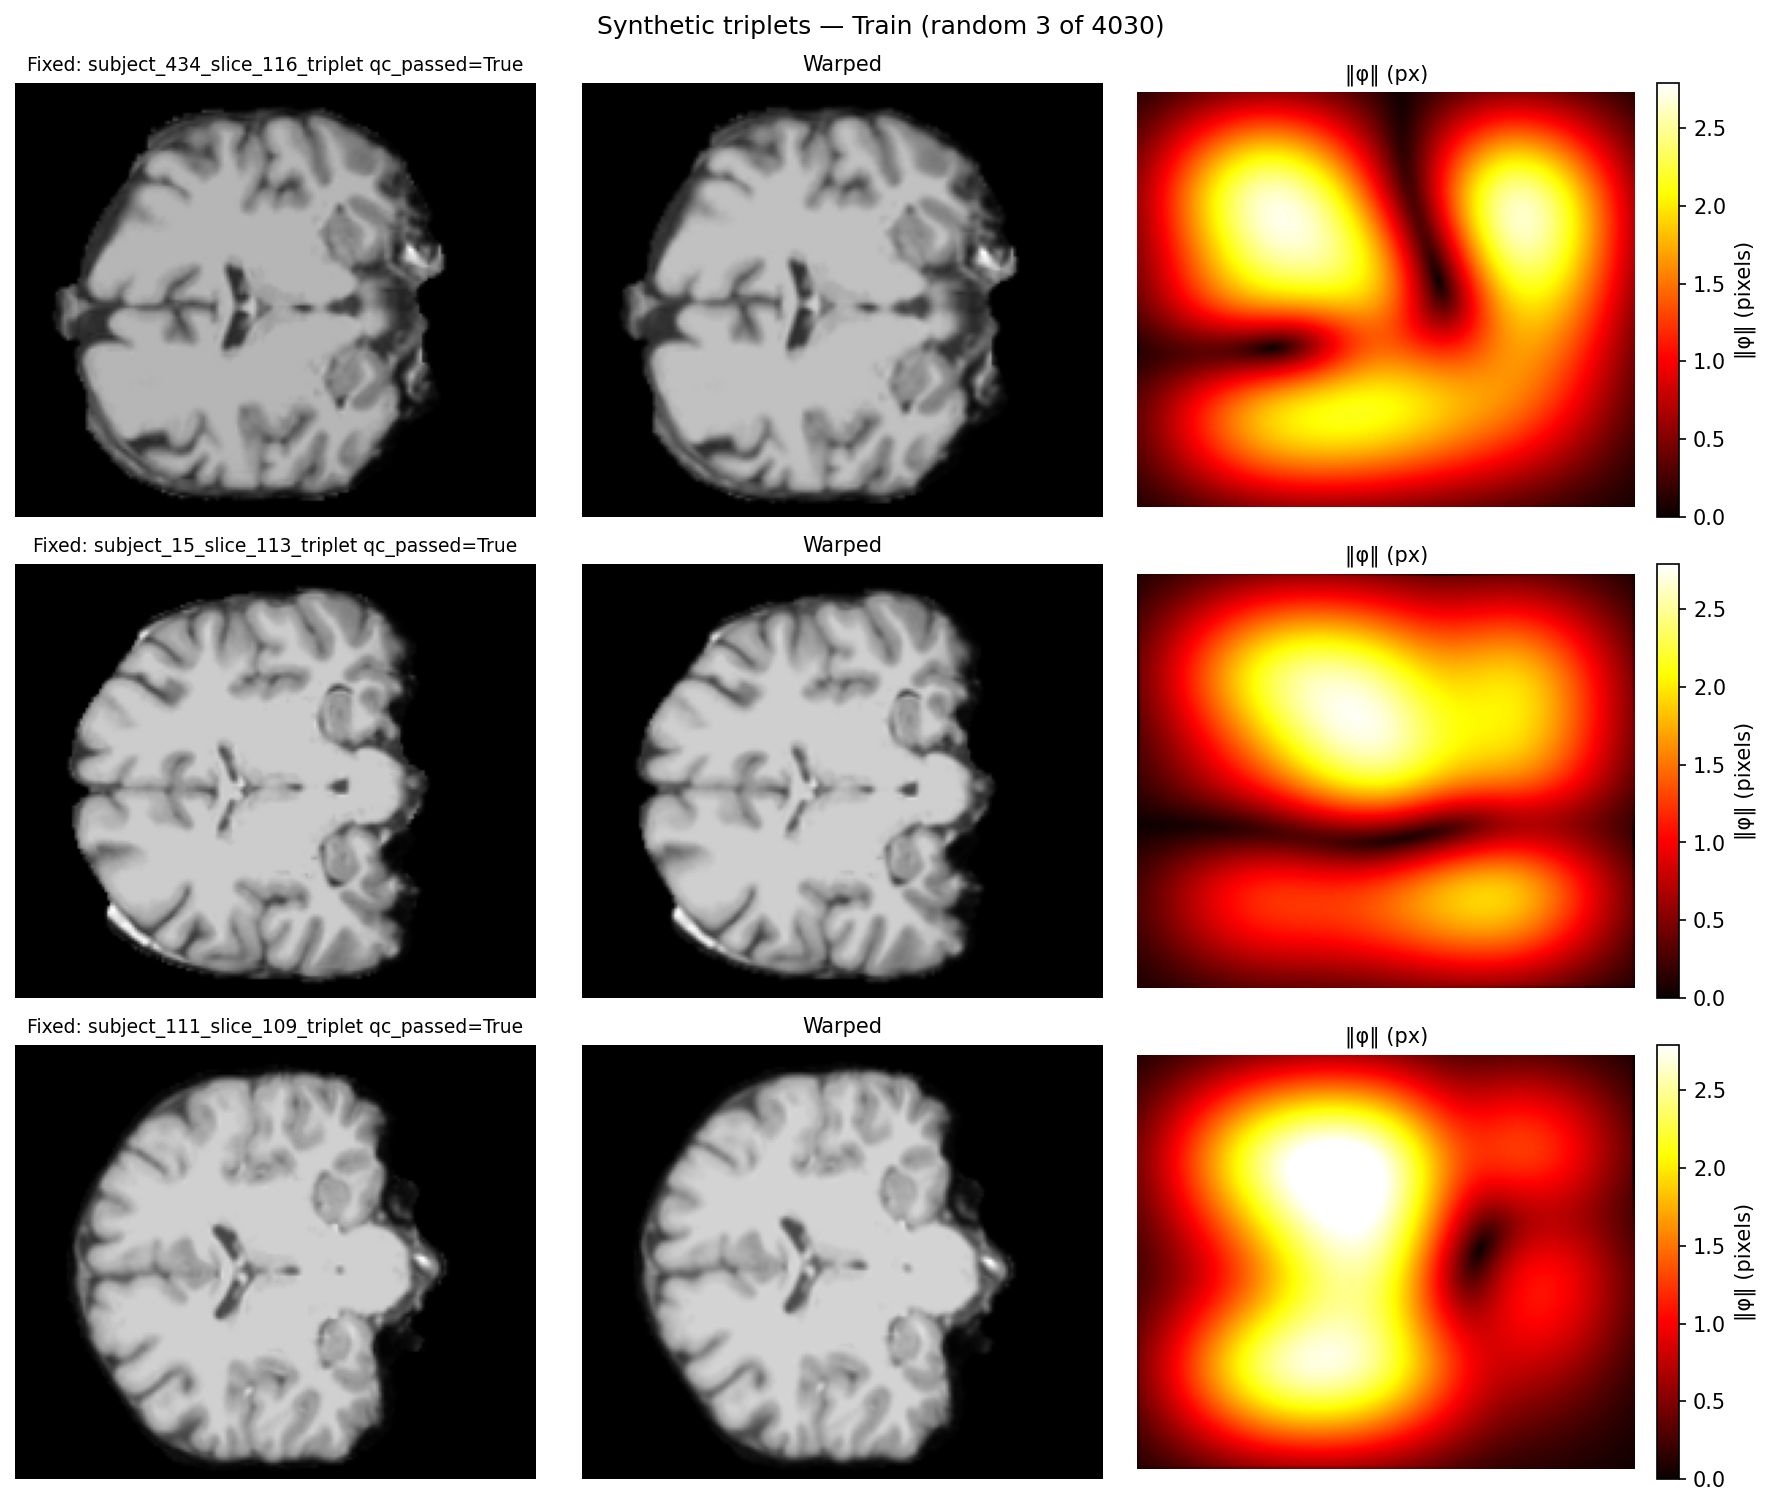
\includegraphics[width=0.95\linewidth]{assets/images/synthetic/ixi_synth_mtrain.png}
  \caption{Synthetic registration triplets generated in Phase~1 (fixed image, warped image, and deformation magnitude $\|\phi\|$).}
  \label{fig:triplet_examples}
\end{figure}

To support qualitative analysis across ``easy'' and ``hard'' deformation regimes, we additionally select min/median/max examples by a scalar $\phi$ statistic (default: mean deformation magnitude over the slice). Figure~\ref{fig:triplet_minmedmax} illustrates these representative extremes.

\begin{figure}[t]
  \centering
  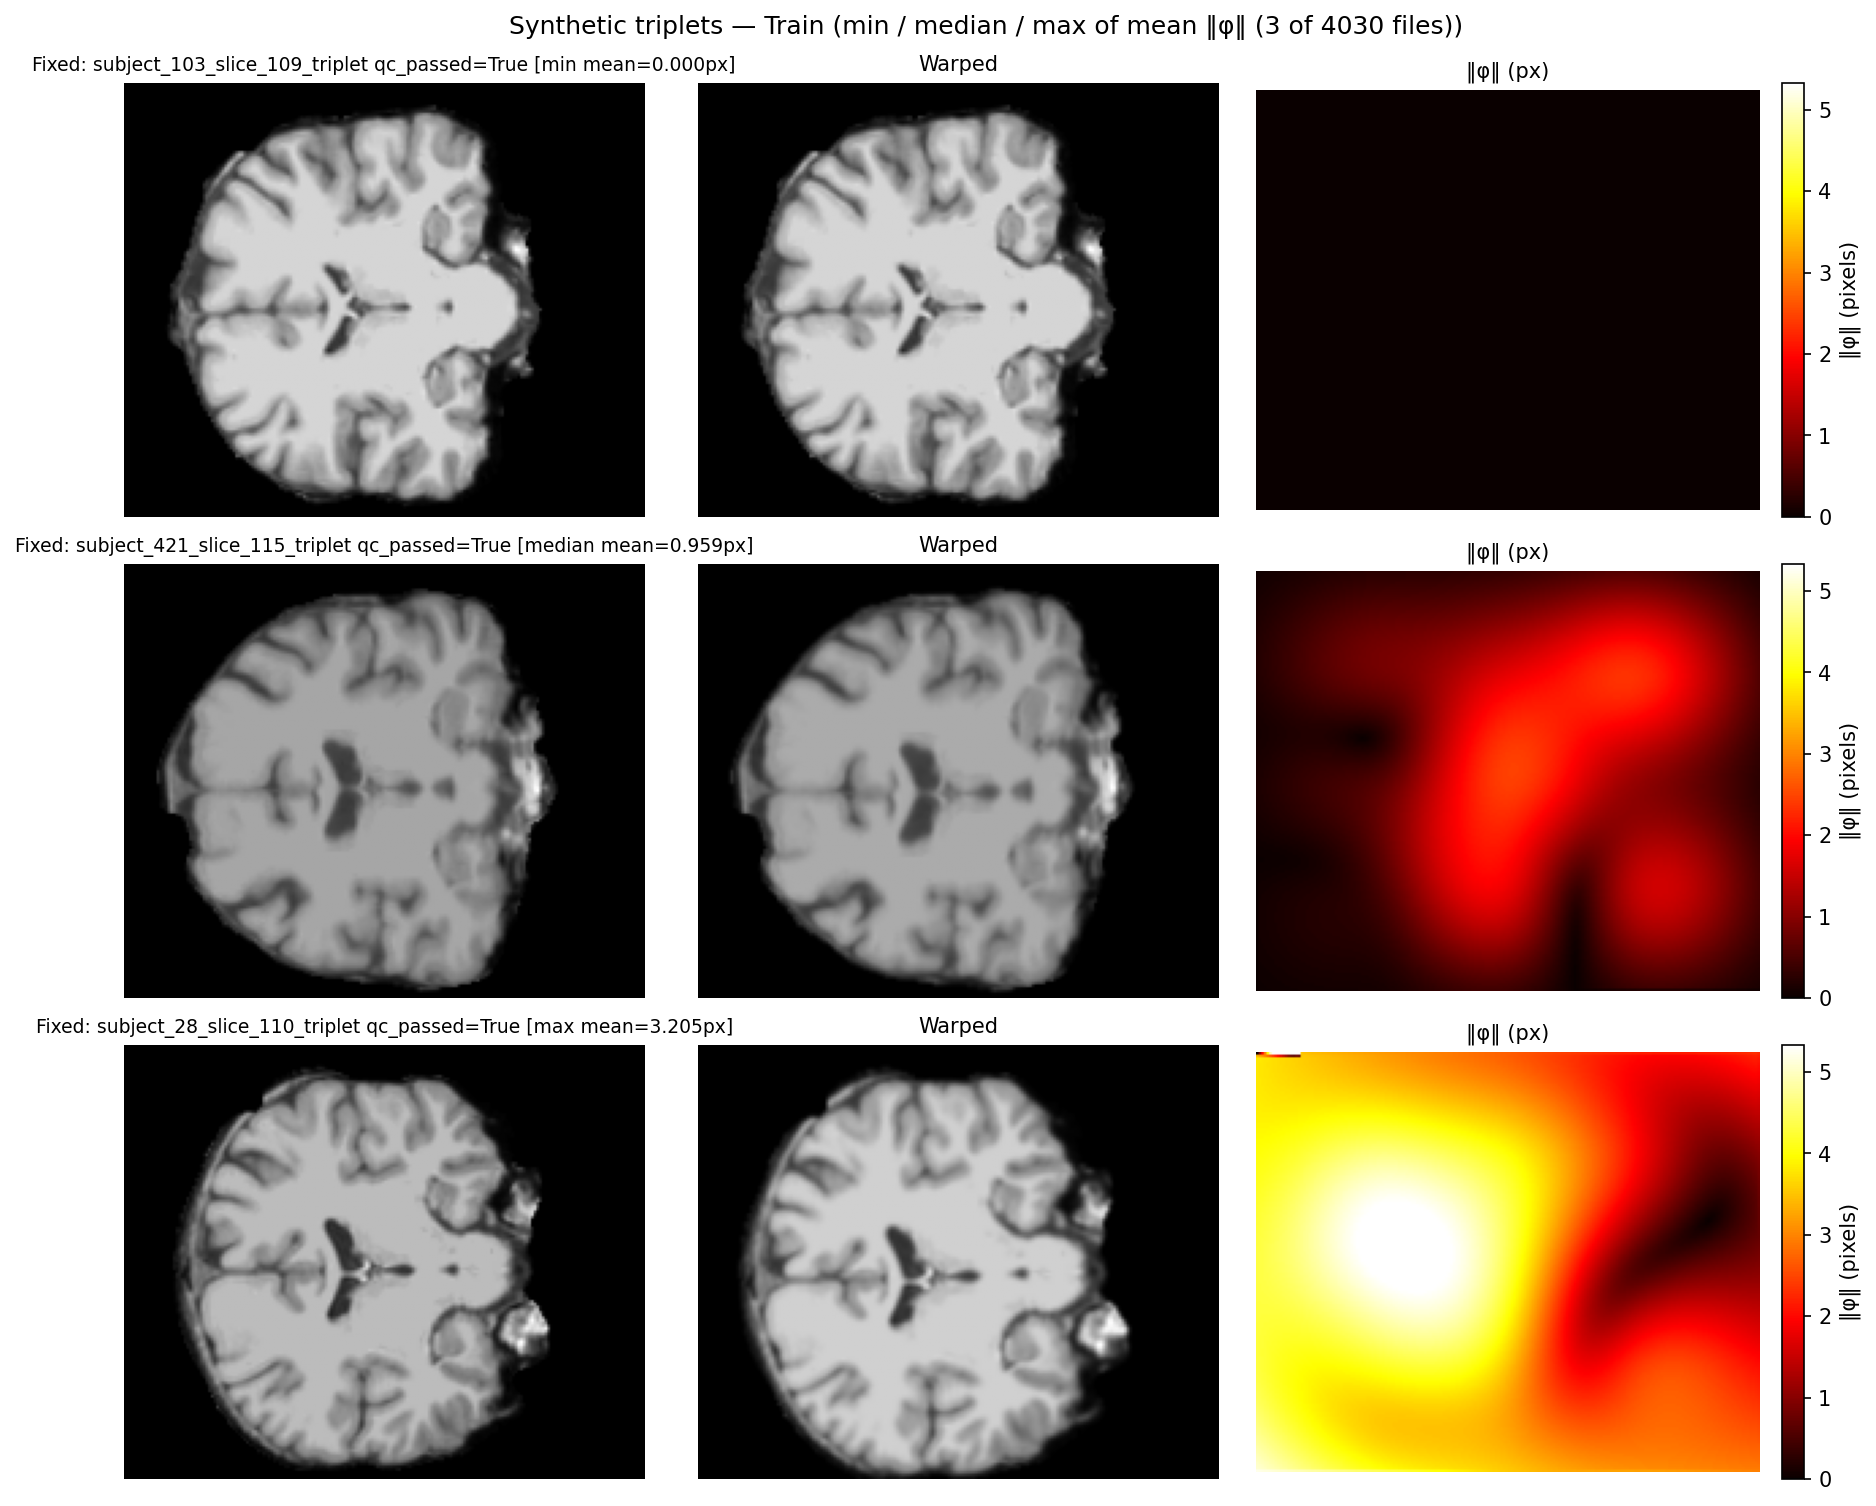
\includegraphics[width=0.95\linewidth]{assets/images/synthetic/ixi_synth_mtrain_minmedmax.png}
  \caption{Min/median/max synthetic triplets by deformation magnitude $\|\phi\|$ for the Train split.}
  \label{fig:triplet_minmedmax}
\end{figure}

\subsection{Phase 2: Registration Error Map Generation}
Phase~2 converts synthetic triplets into supervised scalar error maps by running UniGradICON to predict a deformation field and comparing it with the known synthetic ground truth.

\paragraph{UniGradICON fiver generation.}
For each triplet in each split (Train/Val/Test/Atlas), we:
\begin{itemize}
  \item Run UniGradICON to infer the deformation in the ICON coordinate system.
  \item Convert the predicted deformation back to the original 2D pixel grid to obtain $\phi_{\text{pred}}$ in pixel units.
  \item Compute the residual displacement $\phi_{\text{diff}}=\phi_{\text{true}}-\phi_{\text{pred}}$.
  \item Produce a scalar error map
  \[
    e(u) = \|\phi_{\text{true}}(u) - \phi_{\text{pred}}(u)\|_2
         = \sqrt{\Delta\phi_x(u)^2 + \Delta\phi_y(u)^2}.
  \]
\end{itemize}

The output fiver files ($\ast$$_\mathrm{fiver}$.npz) store, for each pixel, the fixed/warped images, $\phi_{\text{true}}$, $\phi_{\text{pred}}$, $\phi_{\text{diff}}$, and the scalar error map $e(u)$. Importantly, they also store $\mathrm{valid\_mask}$ and the QC flag propagated from Phase~1, enabling masked training later.

\paragraph{Phase~2 visualization.}
Figures~\ref{fig:unigrad_train} and \ref{fig:unigrad_train_minmedmax} show the UniGradICON-derived quantities for representative Train samples, including $\|\phi_{\text{true}}\|$, $\|\phi_{\text{pred}}\|$, and the scalar error map $\|\phi_{\text{true}}-\phi_{\text{pred}}\|$.

\begin{figure}[t]
  \centering
  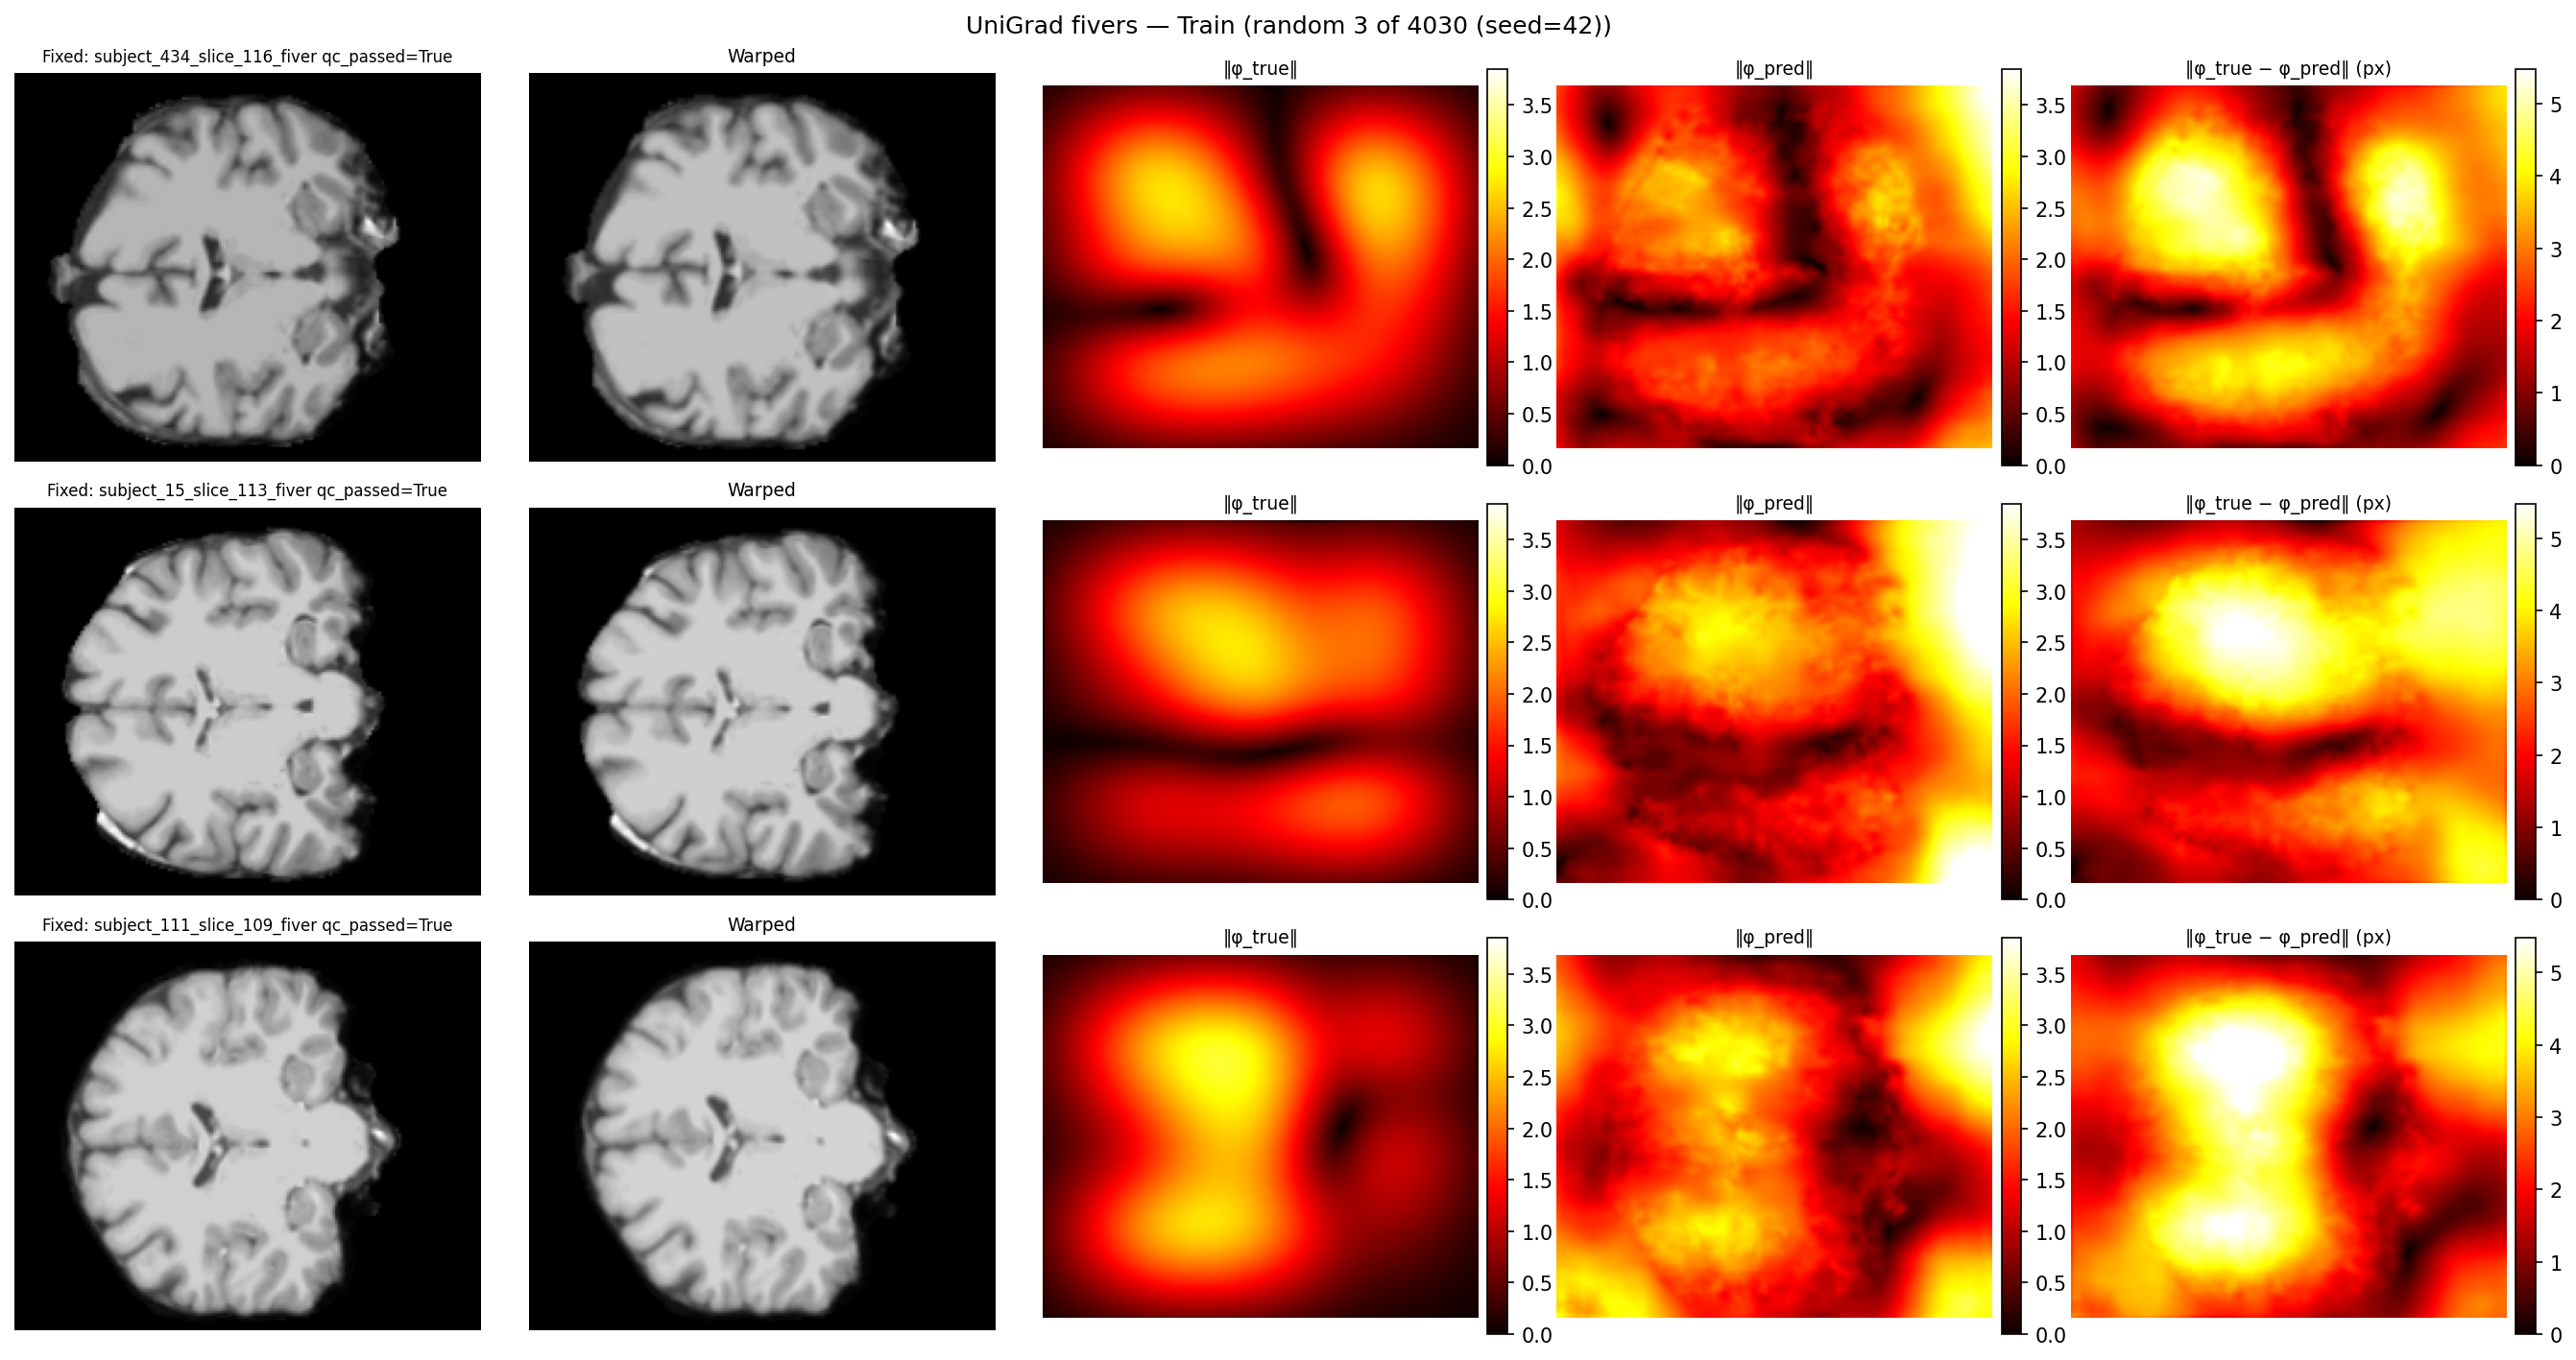
\includegraphics[width=0.95\linewidth]{assets/images/unigrad/ixi_unigrad_train.png}
  \caption{UniGradICON fiver visualization in Phase~2 for the Train split (including $\|\phi_{\text{true}}\|$, $\|\phi_{\text{pred}}\|$, and the scalar error map).}
  \label{fig:unigrad_train}
\end{figure}

\begin{figure}[t]
  \centering
  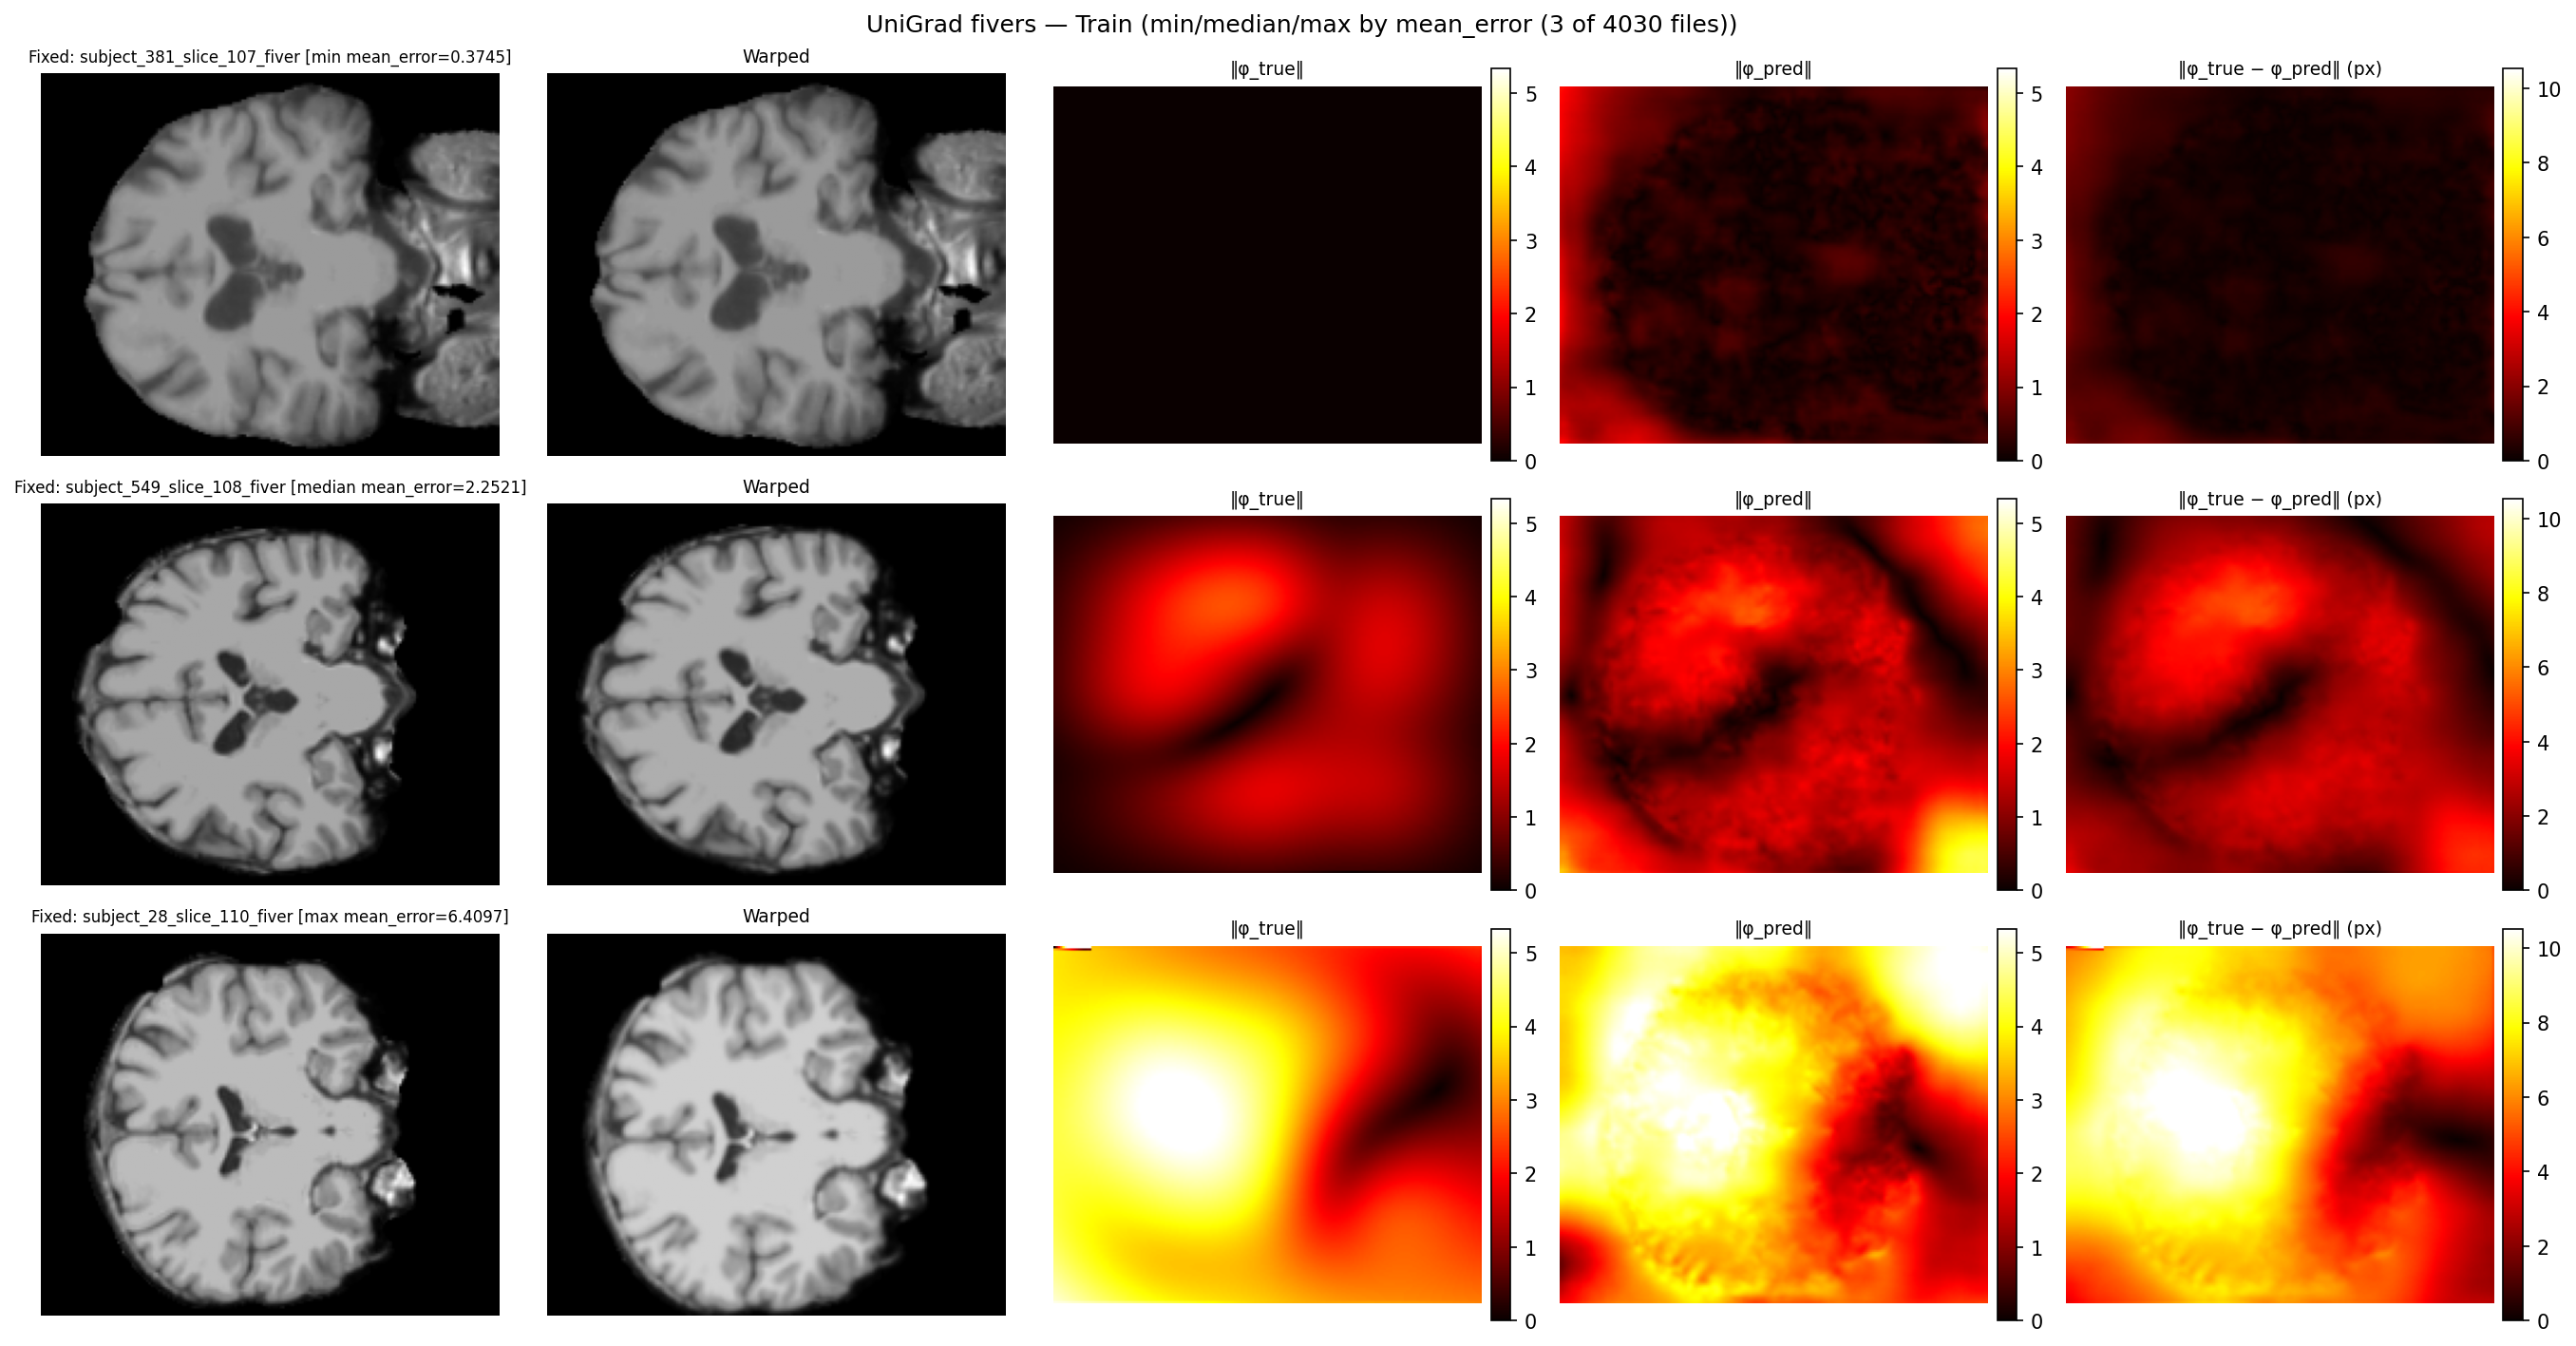
\includegraphics[width=0.95\linewidth]{assets/images/unigrad/ixi_unigrad_train_minmedmax.png}
  \caption{Train split fivers selected by deformation/error extremes (min/median/max) to inspect how predicted displacement magnitude relates to error magnitude.}
  \label{fig:unigrad_train_minmedmax}
\end{figure}

\paragraph{Why error-map supervision helps bypass the Correspondence Paradox.}
By using synthetic ground truth, Phase~2 provides a known pixelwise registration error map. This enables supervised learning of an ``uncertainty proxy'' $\,\hat{e}(u)\,$ using observable inputs and UniGradICON’s predicted deformation field, rather than relying on correspondence uncertainty to generate supervision signals.

\subsection{Phase 3: Supervised Error Map Training}
In Phase~3 we train a 2D U-Net to regress the scalar registration error map $e(u)$ produced in Phase~2.

\paragraph{Model inputs and output.}
Each training sample is built from the UniGrad fiver:
\begin{itemize}
  \item \emph{Input channels:} fixed image $I_{\text{fixed}}$, warped image $I_{\text{warped}}$, and $\phi_{\text{pred}}$ (two displacement components), concatenated into a 4-channel tensor.
  \item \emph{Output:} predicted error map $\hat{e}(u)$ (single channel).
\end{itemize}

In the default configuration, the network also applies per-slice robust intensity normalization to fixed/warped images before learning; $\phi_{\text{pred}}$ is scaled by a constant factor so that the regression operates on consistent pixel-displacement magnitudes.

\paragraph{Masked regression loss.}
Because boundaries can include transform artifacts and correspondences are less reliable near the periphery, training uses $\mathrm{valid\_mask}$ and computes the loss only over valid interior pixels:
\[
  \mathcal{L}_{\text{mse}}
  = \frac{1}{|\Omega_{\text{valid}}|}\sum_{u\in \Omega_{\text{valid}}}\left(\hat{e}(u)-e(u)\right)^2.
\]
This masked loss is implemented as a masked MSE averaged over valid pixels.

\paragraph{Optional boundary smoothness regularization.}
To reduce spurious oscillations near the transition between valid and invalid regions, an optional smoothness term can be added. The regularizer applies a gradient-based penalty to the prediction along edges where supervision is absent (i.e., at invalid regions), controlled by a hyperparameter $\texttt{smooth\_weight}$.

\paragraph{Optimization and checkpoint selection.}
Training uses AdamW with configurable hyperparameters (learning rate, weight decay) and validates after each epoch. We select the best checkpoint by the minimum validation masked MSE, producing a single final model used for evaluation.

\paragraph{Qualitative evaluation and error regime analysis.}
After training, we evaluate qualitative performance by selecting representative fivers from both the Test and Atlas splits. Two selection modes are used:
\begin{itemize}
  \item \emph{Random selection:} pick $N$ random samples from the split.
  \item \emph{Min/median/max selection:} rank samples by a scalar computed as the \emph{mean} error map over the slice. When available, the mean is masked by $\mathrm{valid\_mask}$. We then plot the min/median/max ranked samples to inspect behavior across low- and high-error regimes.
\end{itemize}

This design enables a compact visual analysis of how the predicted displacement magnitude $\|\phi_{\text{pred}}\|$ and the predicted scalar error map $\hat{e}(u)$ evolve across increasing ground-truth error.

\subsection{Summary Table: What Each Phase Produces}
\begin{table}[t]
  \centering
  \begin{tabular}{p{0.28\linewidth} p{0.67\linewidth}}
    \hline
    \textbf{Phase} & \textbf{Main output (data/artefacts)} \\
    \hline
    I. Ground Truth Generation &
    Synthetic $(I_{\text{fixed}}, I_{\text{warped}}, \phi_{\text{true}})$ triplets with
    $\mathrm{valid\_mask}$ and QC flags; deformation magnitude statistics are constrained via QC. \\
    \hline
    II. Error Map Generation &
    UniGradICON-derived $\phi_{\text{pred}}$ and residual displacement $\phi_{\text{diff}}$, producing the supervised scalar error map
    $e(u)=\|\phi_{\text{true}}(u)-\phi_{\text{pred}}(u)\|_2$ and propagating $\mathrm{valid\_mask}$ and QC flags. \\
    \hline
    III. Supervised Training &
    A U-Net regression model trained on masked MSE (and optional boundary smoothness) to predict $\hat{e}(u)$, with a best checkpoint selected by validation masked MSE. \\
    \hline
  \end{tabular}
  \caption{Summary of the three-stage pipeline and the primary supervision artefacts produced at each stage.}
  \label{tab:pipeline_outputs}
\end{table}

